\documentclass[11pt]{article}
% ------------------------------------------------------------------------------------------------
% 생성형 AI를 감당할 수 있는가 -- 국문판 (영문 원고 v2.0의 번역; 컴파일: xelatex, bibtex, xelatex, xelatex)
% 기본 표: code/40_tables_tex.py; v2.0 표: revision_audit/build_revision_tables_ko.py
% (영문 표 본문에서 행 이름만 옮기므로 숫자는 영문판과 같다).
% ------------------------------------------------------------------------------------------------
\usepackage[a4paper,margin=1in]{geometry}
\usepackage{mathptmx}
\usepackage[no-math]{fontspec}
\usepackage{xetexko}
\setmainfont{Liberation Serif}
\setsansfont{Liberation Sans}
\setmonofont{Liberation Mono}
\setmainhangulfont{Noto Serif CJK KR}[ItalicFont={Noto Sans CJK KR}, BoldFont={Noto Serif CJK KR Bold}, BoldItalicFont={Noto Sans CJK KR Bold}]
\setsanshangulfont{Noto Sans CJK KR}
\setmonohangulfont{Noto Sans CJK KR}
\usepackage{amsmath,amsthm}
\usepackage{booktabs,threeparttable,tabularx,array,multirow}
\usepackage{graphicx}
\usepackage[labelfont=bf,font=small,skip=4pt]{caption}
\usepackage{setspace}
\usepackage[authoryear,round]{natbib}
\usepackage{xcolor}
\usepackage{enumitem}
\usepackage{placeins}
\usepackage[hidelinks]{hyperref}
\usepackage{xurl}
\urlstyle{same}  % URLs in the text font (no bitmap typewriter fonts)
\setstretch{1.35}
\setlist{itemsep=2pt,topsep=4pt}
\setlength{\emergencystretch}{2em}
\newtheorem{proposition}{명제}
\theoremstyle{definition}
\newtheorem{definition}{정의}
\theoremstyle{remark}
\newtheorem{remark}{비고}
\renewcommand{\proofname}{증명}
\newcommand{\AAB}{\mathit{AAB}}
\makeatletter\newcommand{\tabinput}[1]{\@@input #1 }\makeatother % primitive input: safe inside tabular
\providecommand{\doi}[1]{\url{https://doi.org/#1}}
\captionsetup[table]{name=표}
\captionsetup[figure]{name=그림}
\renewcommand{\refname}{참고문헌}
\renewcommand{\abstractname}{초록}

\title{\textbf{생성형 AI를 감당할 수 있는가:\\ 국가 간 균일한 가격과 불균등한 부담}}
\author{오태환\thanks{독립연구자, 대한민국. ORCID: \href{https://orcid.org/0009-0004-4111-4802}{https://orcid.org/0009-0004-4111-4802}. 전자우편: \href{mailto:noah.taehwan@gmail.com}{noah.taehwan@gmail.com}. 자료와 코드: \href{https://doi.org/10.5281/zenodo.23006365}{https://doi.org/10.5281/zenodo.23006365}(재현성 패키지 전체 버전, 부록~\ref{app:data} 참조). 이 논문의 이전 판은 SSRN 워킹페이퍼 7535900으로 공개되었다. 이 판: \mbox{2026년 9월 30일}. 이 글은 영문 원고 \textit{Affording Generative AI Across Countries: Uniform Prices, Unequal Burdens}의 국문판이다. 영문판이 원본이며, 내용과 수치는 같다.}}
\date{2026년 9월}

\begin{document}
\maketitle

\begin{abstract}
\noindent 소비자용 생성형 AI는 나라마다 거의 같은 구독 메뉴로 판매되지만, 국민소득은 나라에 따라 100배 수준으로 차이 난다. 이 논문은 현지 가격이 그 차이에 얼마나 맞춰지는지 측정한다. 하루 동안 170개 국가별 애플 앱스토어에서 ChatGPT, Claude, Gemini의 9개 요금제에 표시된 세금 포함 현지 가격을 조사하고, 201개 경제권에서 각 요금제의 연간 비용을 1인당 GNI 대비 비율로 계산한다. 20달러 표준 요금제의 가격은 거의 균일하다. 현지 달러 가격의 소득 기울기는 0.03--0.04이며, 가격이 현지 물가수준을 따른다면 이 값은 0.23이 된다. 부분적으로라도 현지화된 것은 OpenAI의 입문 요금제뿐이며(기울기 0.14), 저소득국의 앱스토어는 모두 미국 달러로 가격을 매긴다. 그 결과 20달러 요금제의 연간 비용은 고소득국 중위값에서 1인당 소득의 0.65\%, 저소득국 중위값에서 29\%이고, 분석 대상 경제권의 생산가능인구 중 60\%는 이 비용이 광대역에 적용되는 2\% 기준을 넘는 곳에 산다. 두 공개 이용 지표는 소득 기울기가 서로 다르다. 생성형 AI 이용 여부는 0.37, 1인당 Claude 이용량은 0.71이다. 이 대비는 무료 요금제가 최초 채택을 유료 가격에서 분리한다는 모형과 부합하지만, 그 모형을 검정하지는 않는다. 또한 숙련도가 낮은 이용자의 생산성 이익이 더 크다는 사실은, 노출도와 채택이 함께 따라가지 않는 한 국가 간 수렴을 뜻하지 않는다. 이 조사는 하루 동안의 표시가격 스냅샷이며, 이 논문은 가격·접근 정책을 평가하려면 무엇이 필요한지 제시한다.

\medskip
\noindent\textbf{주제어:} 생성형 AI; 적정부담(affordability); 디지털 격차; 국제 가격차별; 기술 확산; 경제발전\\
\noindent\textbf{JEL 분류:} O33, O15, L11, L86, D63, F63
\end{abstract}

\newpage
% ================================================================================================
\section{서론}\label{sec:intro}

현장·실험 연구는 생성형 AI가 생산성을 높이며, 그 이익이 경험이 적은 근로자에게 가장 크게 돌아가는 경우가 많음을 시사한다 \citep{brynjolfsson2025generative,noy2023experimental,dellacqua2023navigating,peng2023impact}. 다만 이 결과는 이미 AI를 쓸 수 있었던 사람들에 관한 것이다. 같은 기회가 나라마다 주어지는지는 먼저 사람들이 그 도구를 쓸 수 있는지에 달려 있다. 그런데 프런티어 역량은 전 세계적으로 표준화된 메뉴의 구독 상품으로 개인에게 판매된다. 무료 요금제, 월 20달러 표준 요금제, 그리고 약 100달러와 200달러의 고사용량 요금제다(표~\ref{tab:ladder}). 같은 달러 가격도 소득에 따라 무게가 크게 다르다. 월 20달러는 미국에서 1인당 소득의 0.3\%이지만 모잠비크에서는 40\%를 넘는다.

이 논문은 현지 구독 가격이 국민소득의 차이에 얼마나 맞춰지는지, 그리고 균일한 가격이 나라별 생성형 AI의 감당 가능성에 어떤 의미를 갖는지 묻는다. 이 논문의 기여는 날짜가 명시된 여러 사업자의 현지 가격 조사다. 2026년 9월 27일 하나의 결제 경로에서 모든 애플 앱스토어 국가별 스토어(218개 코드, 이 중 170개에 현지 가격 목록)를 대상으로 ChatGPT, Claude, Gemini의 9개 요금제에 표시된 세금 포함 가격을 수집하고, 201개 경제권에서 각 요금제의 연간 비용을 1인당 GNI 대비 비율로 계산했다. 선행 연구는 ChatGPT Plus의 20달러 요금을 국민소득과 비교했다 \citep{sathish2024llempower}. 이 조사는 여기에 미국 가격이 아닌 현지 가격, 여러 사업자와 요금 단계, 그리고 수집 결과·통화·요금제 매칭의 기록을 더한다. 각 스토어 안에서 ChatGPT Go와 Plus를 짝지어 비교해, 입문 요금제에 관한 결과가 환율 환산에 좌우되지 않는지도 점검한다.

결과는 네 가지다. \emph{표준 요금제의 가격은 거의 균일하다.} 국가별 스토어 전체에서 현지 달러 가격의 소득 기울기는 ChatGPT Plus 0.039, Claude Pro 0.026, Google AI Pro 0.037이다. 가격이 현지 물가수준을 따른다면 이 값은 0.23, 소득에 비례한다면 1이 된다. \emph{부분적으로라도 현지화된 것은 OpenAI의 입문 요금제뿐이다.} ChatGPT Go의 기울기는 0.143으로, 물가수준 기울기의 약 60\%이자 비례 가격의 7분의 1이다. Google의 입문 요금제는 고소득국을 뺀 모든 소득집단에서 4.99달러로 표시된다. 저소득국의 앱스토어는 모두 미국 달러로 가격을 매기며, 저소득국의 36\%에는 현지 스토어가 아예 없다. \emph{따라서 부담은 소득에 따라 가파르게 기울어 있다.} 20달러 요금제의 연간 비용은 고소득국 중위값에서 1인당 소득의 0.65\%, 상위중소득국 3.1\%, 하위중소득국 8.7\%, 저소득국 29\%다. 이 요금제는 1인당 소득이 12,000달러 이상인 곳에서만 ITU와 유엔 광대역위원회가 광대역에 적용하는 2\% 기준을 충족하며, 분석 대상 경제권의 생산가능인구 중 60\%는 그렇지 않은 곳에 산다. 저소득국 중위 경제에서는 가장 부유한 20\% 가구에게도 요금제 하나의 비용이 평균소득의 13\%에 이른다. \emph{공개 이용 지표들은 소득 기울기가 서로 다르다.} 어떤 생성형 AI 제품이든 이용하는 성인의 비중에 관한 마이크로소프트 추정치의 소득탄력성은 0.37이며, 그 절반가량은 인터넷 이용의 소득 기울기와 겹친다. 1인당 Claude 이용량에 관한 Anthropic 지수의 소득탄력성은 같은 96개 경제권에서 0.71이며, 이 가운데 저소득국은 한 곳뿐이다.

간단한 분석 틀이 이 사실들을 정리해 준다. 비이용, 무료 이용, 유료 이용의 세 선택지 모형에서, 유료 전환의 문턱이 무료 채택의 문턱보다 높으면 무료 요금제는 AI를 쓸지 말지의 결정을 유료 가격과 분리한다. 이때 유료 마진은 가격이 현지화되지 않는 한 소득 기울기를 그대로 물려받는다(부록~\ref{app:tiermodel}). Claude 이용량의 더 가파른 기울기는 이 메커니즘과 부합하지만, 국가 간 자료로는 이를 식별할 수 없다. 사업자 선택, 이용자당 대화 수, 측정 과정도 같은 순서를 만들어 낼 수 있고, 이 지수는 무료와 유료 계정을 합산하기 때문이다. 두 번째 결과는 수렴에 관한 것이다. 총량 이익은 과업 단위 이익뿐 아니라 노출도와 채택에도 달려 있으므로, 숙련도가 낮은 이용자의 조건부 이익이 더 크다는 사실은 AI가 국가 간 격차를 줄이기 위한 필요조건도 충분조건도 아니다(명제~\ref{prop:equal}). 노출도와 채택의 대략적인 대리변수를 쓰면, 과업 단위 이익이 같을 때 격차를 줄이려면 저소득국 채택률이 약 100\%에 이르러야 하고, 저소득국의 이익이 1.5--2배 크더라도 50--67\%가 필요하다. 현재 저소득국 채택률은 약 9\%다.

이 논문은 여러 갈래의 문헌과 연결된다. 국가 내 생성형 AI 채택 연구는 채택이 젊고 교육 수준이 높으며 소득이 높은 집단에 치우쳐 있음을 보였고 \citep{bick2024rapid,humlum2025unequal}, 웹 트래픽·원격측정(telemetry)·대화 자료를 이용한 국가 간 연구는 소득에 따른 큰 격차를 보고해 왔으며 \citep{liu2024who,liu2025who,misra2025measuring,chatterji2025how,appel2025uneven,daepp2026how,iscenko2026atlas}, 무료 이용과 유료 이용을 구분하는 직접 조사도 나오기 시작했다 \citep{kanzamanova2026digital}. 컴퓨터, 인터넷, 이동통신에 관한 과거 연구는 소득, 인적자본, 가격을 확산의 주된 상관요인으로 보았다 \citep{caselli2001cross,chinn2007determinants,aker2010mobile,bjorkegren2019adoption}. 확산 문헌은 오래전부터 채택 시점과 이용 강도를 구분해 왔으며 \citep{comin2004cross,comin2010exploration}, \citet{comin2018technology}는 과거 기술에서 채택 시차는 국가 간에 수렴했지만 이용 강도는 발산했음을 보였다. AI의 직업별 노출 연구 \citep{felten2021occupational,eloundou2024gpts,cazzaniga2024genai,gmyrek2025generative}는 아래에서 쓰는 노출도 수치를 제공하고, 개발 관점의 평가 \citep{korinek2021artificial,undp2025hdr,unctad2025tir,worldbank2026wdr}는 정책적 함의를 논의하는 틀이 된다. 통신 적정부담 관행 \citep{itu2025ff}은 이 논문이 AI로 넓혀 적용하는 기준을 제공하며, 국제 가격 결정과 제품 버저닝 문헌 \citep{goldberg1997goods,cavallo2014currency,mussa1978monopoly,goldfarb2019digital}은 현지 가격 조사를 해석하는 틀이 된다. 다만 세금, 플랫폼 수수료, 제품 차이 때문에 추정된 기울기를 기업의 가격차별 모수로 볼 수는 없다.

이 분석은 기술(記述)적이다. 달러 가격이 균일하면 부담은 소득의 단조변환이 되므로, 부담과 이용 사이의 국가 간 연관성으로는 가격 효과를 식별할 수 없다. 또한 가격 조사는 이용 자료의 측정 기간보다 늦고, 하나의 결제 경로를 하루 동안 관찰한 것이다. 현지화된 입문 요금제의 단계적 출시와 조사 이틀 뒤 OpenAI가 발표한 요금 변경 덕분에 이제 평가 설계가 가능해졌으며, 제~\ref{sec:discussion}절은 그 설계에 필요한 조건을 제시한다.

제~\ref{sec:background}절은 가격 메뉴와 그 뒤의 요금 변경을 설명한다. 제~\ref{sec:model}절은 부담 지표를 정의하고 분석 틀을 제시한다. 제~\ref{sec:data}절은 자료를 설명하고, 제~\ref{sec:results}절은 가격 조사, 부담, 이용 지표 비교의 결과를 보고한다. 제~\ref{sec:discussion}절은 해석, 평가 설계, 정책, 한계를 논의하며, 제~\ref{sec:conclusion}절에서 결론을 맺는다. 형식 모형, 자료 구축, 연결성 분해, 추가 표, 500달러 기준 요금 시나리오, 측정 프로토콜은 부록에 수록하였다.

% ================================================================================================
\section{가격 메뉴}\label{sec:background}

표~\ref{tab:ladder}에는 2026년 9월 27일 각 사업자의 공식 페이지에 게시된 대표적 AI 비서 세 곳의 소비자 요금제와, 같은 요금제의 미국 앱스토어 가격을 정리하였다. 가격 회귀는 모두 그날의 앱스토어 스냅샷을 쓴다. 뒤에서 분석하는 이용 자료의 측정 기간은 2026년 5월이나 6월에 끝나므로, 조사한 가격은 이용 자료보다 나중 시점이다. 메뉴에서는 세 가지 특징이 두드러진다.

\begin{table}[t]
\centering
\begin{threeparttable}
\caption{대표적 AI 비서 세 곳의 소비자 가격 사다리 (2026년 9월)}\label{tab:ladder}
\small
\begin{tabularx}{\textwidth}{@{}l>{\raggedright\arraybackslash}X>{\raggedright\arraybackslash}X>{\raggedright\arraybackslash}X@{}}
\toprule
단계 & OpenAI (ChatGPT) & Anthropic (Claude) & Google (Gemini) \\
\midrule
무료 & 무료 & 무료 & 무료 \\
입문 & Go: \$8 [\$8.00]; 2025년 8월 인도 출시, 170개국 추가 확대, 2026년 1월 미국 출시; 광고 시험 & --- & AI Plus: [\$4.99] \\
표준 & Plus: \$20 [\$19.99] & Pro: 월 \$20, 연간 결제 시 월 \$17 [\$20.00] & AI Pro: [\$19.99] \\
고사용량 & Pro \$100: Plus의 5배 사용량 [\$100] & Max: ``\$100부터'', Pro의 5배 또는 20배 사용량 [\$124.99; \$249.99] & AI Ultra \$100: Pro의 5배 사용량 \\
최고사용량 & Pro \$200: Plus의 20배 사용량 [\$200]; 2026년 9월 10일부터 신규 가입 일시중단 & (Max 20배, 위 참조) & AI Ultra \$200 (종전 \$250): Pro의 20배 사용량 [\$199.99] \\
\bottomrule
\end{tabularx}
\begin{tablenotes}[flushleft]\footnotesize
\item \emph{주:} 2026년 9월 27일 기준 미국 공식 웹 가격(월). 대괄호는 같은 날의 미국 앱스토어 가격(판매세 제외). 웹 가격과 사용량 배수는 참고용이며, 국가 간 회귀에는 앱스토어 기록만 쓴다. OpenAI는 ``두 Pro 요금제는 핵심 기능이 같고 주된 차이는 사용 허용량''이라고 설명한다 \citep{openai2026pro}. Plus 가격과 API 별도 과금은 \citet{openai2026plus}, Go는 \citet{openai2026go}. Anthropic: \citet{anthropic2026pricing}(세금 제외 가격). Google: 2026년 5월 19일 월 100달러 Ultra 신설과 200달러 Ultra(종전 250달러) 발표 \citep{google2026io}. Google 요금제 페이지는 지역별로 다른 가격을 표시하므로 AI Plus와 AI Pro는 대괄호의 앱스토어 가격만 표기하였다. OpenAI의 요금 조건은 2026년 9월 29일에 바뀌었다(제~\ref{sec:tariff}절).
\end{tablenotes}
\end{threeparttable}
\end{table}

\emph{수렴.} 세 사업자의 메뉴는 무료 요금제, 5--8달러의 입문 요금제, 20달러 표준 요금제, 약 100달러와 200달러 요금제로 이루어진 거의 같은 단계로 수렴했다. 여러 AI 비서를 함께 쓰면 비용도 그만큼 늘어난다. 세 서비스의 20달러 요금제를 모두 유지하는 전문직은 월 약 60달러를 낸다.

\emph{지능이 아니라 사용량.} 상위 단계는 주로 사용 허용량(표준 요금제의 ``5배''와 ``20배'')으로, 부차적으로는 최상위 모델과 기능을 쓸 수 있는지로 구분된다. 디지털 재화는 복제의 한계비용이 거의 0이지만 추론 비용은 무시할 수 없으므로 버저닝(versioning)에 적합하며 \citep{goldfarb2019digital}, 이 메뉴는 수량과 품질에 따른 2급 가격차별의 전형이다 \citep{mussa1978monopoly}. 무료 요금제와 입문 요금제는 표준 요금제의 품질을 낮춘 판본이다. 예컨대 ChatGPT Go는 사용 한도가 낮은 ``Instant'' 모델을, Plus는 한도가 높은 ``Thinking'' 모델을 제공한다 \citep{openai2026go}. 따라서 더 높은 가격은 한 달에 쓸 수 있는 프런티어 역량을 더 많이 산다. 다만 요금제 이름도 가격도 사업자, 언어, 과업에 걸쳐 쓸모 있는 역량을 비교할 수 있는 척도는 아니다.

\emph{현지화는 사다리의 맨 아래에서 일어난다.} 입문 요금제는 사업자가 소득이 낮은 시장에 다가가는 수단이다. ChatGPT Go는 2025년 8월 인도에서 출시된 뒤 170개국으로 추가 확대되었고, 2026년 1월 미국에서 8달러에 출시되었다 \citep{openai2026go}. 제~\ref{sec:prices}절은 이것이 현지 가격이 소득에 따라 의미 있게 달라지는 유일한 단계임을 보인다. 인도에서 이동통신 가입과 결합해 프리미엄 요금제를 무상으로 주는 판촉처럼, 일부 시장에서는 판촉이 실효 가격을 더 낮춘다. 그러나 이러한 판촉은 한시적이고 국가별로 다르며, 표시가격 조사에는 잡히지 않는다.

\subsection{2026년 9월 29일의 요금 변경}\label{sec:tariff}

조사 이틀 뒤 OpenAI는 월 500달러의 Pro 500 요금제를 발표했다. 이 요금제는 처음에는 웹에서 판매되며 가장 빠른 서비스 모드를 포함한다. OpenAI는 동시에 Pro 200의 신규 가입을 다시 열면서 신규 가입자의 기본 사용 허용량을 낮췄고, 기존 가입자는 2026년 10월 29일까지 종전 허용량을 유지한다 \citep{openai2026releasenotes,openai2026prorevision}. 이 사례는 측정에 관한 두 가지 점을 보여 준다. 요금이 같아도 가입 시점과 날짜에 따라 이용 권리가 다를 수 있고, 새 요금제는 기존 가격을 대체하는 대신 이용 자격을 더할 수 있다. 따라서 요금 조건은 요금, 기본 허용량, 이용 가능한 모델과 서비스 모드, 초과 사용 조건, 초기화 규칙의 묶음 $(F,\mathbf{A},\mathcal{E},\mathbf{r},\mathbf{w})$이며, 아래에서 정의하는 부담은 이 가운데 요금 $F$만을 쓴다. 모델 시장의 품질 조정 가격은 빠르게 떨어진다 \citep{andre2025markets}. 그러나 이 가격은 구독의 반복적인 현금 지출과는 다른 대상이며, 어느 쪽도 특정 과업을 완료하는 데 드는 현금 비용을 알려 주지 않는다. 이 변경은 가격 조사와 이용 자료 측정 기간보다 모두 늦으므로 따로 다룬다. 부록~\ref{app:500}은 500달러 기준 요금 시나리오를, 부록~\ref{app:protocol}은 요금만으로는 빠지는 요금 조건의 요소를 기록하는 프로토콜을 제시한다.

% ================================================================================================
\section{분석 틀}\label{sec:model}

\subsection{적정부담 지표}

\begin{definition}[AI 적정부담 지표]
국가 $c$에서 월 가격이 $p_c$(현재 달러)인 요금제와 1인당 소득 $y_c$(현재 달러)에 대하여
\begin{equation}
\AAB_c(p_c) = \frac{12\,p_c}{y_c}\times 100 .
\label{eq:aab}
\end{equation}
\end{definition}

이 부담은 정규화된 가격이다. 가격이 평균소득에 비해 얼마나 큰지를 나타낼 뿐, 지출 비중이 아니며 누군가가 실제로 얼마를 쓰는지를 측정하지도 않는다. 분모는 3년간의 환율을 평활하는 Atlas 방식 1인당 GNI다. 이 지표는 ITU의 광대역 적정부담 통계 관행을 따른다. ITU는 입문 수준 바스켓의 월 가격을 월 1인당 GNI 대비 비율로 나타내고, 이를 유엔 광대역위원회의 2\% 기준에 비추어 평가한다 \citep{itu2025ff}. 이 논문은 그 기준을 빌려 온 참조선으로 쓰고, 다른 기준값에 대한 민감도도 보고한다. 기준값을 $t$(퍼센트포인트)라 하면 문턱 소득은 $y_c\geq1200p/t$이며, 2\%에서는 20달러 요금제의 경우 12,000달러, 8달러 요금제의 경우 4,800달러다.

평균소득은 분배를 가리므로 소득 5분위 평균에서의 부담도 계산한다. 분위 $q$의 평균소득은 $y_{cq}=y_c s_{cq}/0.2$로 근사하며, $s_{cq}$는 가계조사에 기초한 그 분위의 소득 또는 소비 점유율이다. 가계조사의 후생 개념, 조사 시점, 국민계정이 서로 다르므로 이 값은 측정된 가처분소득이 아니라 합성된 자원 수준이다. 또한 GNI에는 가계에 귀속되지 않는 소득도 들어 있으므로 1인당 가계최종소비지출 대비 부담도 함께 보고한다.

\begin{remark}[PPP 분모가 측정하는 것]\label{rem:ppp}
달러로 가격이 매겨진 서비스라면 시장환율 기준 소득 대비 부담이 현금 비용으로서 적절한 양이다. 달러 가격을 구매력평가(PPP) 소득으로 나누면 대신 $12p/y^{PPP}_c = 12\,(p\cdot PLR_c)/y_c$가 된다. 여기서 Atlas 소득과 PPP 소득의 비율인 $PLR_c = y_c/y^{PPP}_c$는 미국 대비 물가수준의 대리지표다.\footnote{Atlas 방식은 3년간의 환율을 평균하므로, 197개 경제권에서 이 비율은 같은 해 GDP 물가수준비율과 중위값 3.1\%(90백분위 8.3\%)만큼 차이가 난다. 이 비율의 소득탄력성은 0.228이며, GDP 물가수준비율은 0.224다.} 같은 식은 구성된 가격 $p_c=p\cdot PLR_c$ 아래의 Atlas 소득 기준 부담, 곧 사업자가 가격을 현지 물가수준에 연동했을 때의 부담과 같다. 물가수준은 소득과 함께 오르고 \citep{balassa1964purchasing,samuelson1964theoretical}, PPP 환산계수는 국제적으로 가격이 매겨지는 디지털 서비스가 아니라 폭넓은 소비 바스켓을 위해 설계되었다 \citep{deaton2010understanding}. 그러므로 PPP 기준 비율은 같은 양에 대한 강건성 점검이 아니라 이 반사실적 가격 시나리오로 읽는 것이 적절하다. 제~\ref{sec:prices}절에서 실제 가격을 이 시나리오와 비교한다.
\end{remark}

\subsection{무료 요금제와 접근의 두 마진}\label{sec:mechanism}

무료 요금제는 처음 쓰는 것을 가능하게 하고, 유료 요금제는 더 많은 역량을 제공한다. 부록~\ref{app:tiermodel}의 세 선택지 모형에서 연결된 개인은 서로 다른 가치평가를 바탕으로 비이용, 무료 이용, 유료 이용 가운데 하나를 고른다. 유료 전환의 문턱이 무료 요금제 이용의 문턱보다 높으면, AI를 쓸지 말지는 연결성, 숙련, 언어 같은 비금전적 장벽이 결정하고 유료 가격은 이 결정에서 빠진다. 반면 더 많은 역량에 돈을 낼지는 소득 대비 가격에 달려 있다. 따라서 부록~\ref{app:tiermodel}의 명제~\ref{prop:margins}는 가격이 현지화되지 않는 한 유료 마진의 소득 기울기가 이용 여부 마진보다 가파르고, 현지화가 커질수록 그 차이가 줄어든다고 예측한다. 유료 선택지가 비이용자를 곧바로 끌어올 만큼 매력적이면 유료 가격은 두 마진 모두에 영향을 준다. 이 모형은 공통의 참여 비용과 서비스 수준을 조건으로 한다. 모형은 증거를 정리하고 예측을 내놓지만, 공개 이용 자료는 유료 전환을 관측하지 못하므로 아래에서 모형을 추정하거나 검정하지는 않는다.

\subsection{조건부 이익과 무조건부 격차}\label{sec:equal}

AI가 경제 $i$의 산출을 $\Delta Y_i/Y_i = s_L E_i a_i g_i$만큼 늘린다고 하자. 여기서 $s_L$은 노동소득분배율, $E_i$는 AI에 노출된 노동 과업의 비중, $a_i$는 노출 과업에서의 채택률, $g_i$는 과업 단위 생산성 향상률이며, 이는 헐튼 방식의 회계를 AI에 적용한 것이다 \citep{hulten1978growth,acemoglu2019automation,acemoglu2025simple}. 근로자 1인당 산출이 $y_H>y_L$인 두 경제(또는 집단) $H$와 $L$에서 상대 격차는 $R_0=y_H/y_L$에서 다음으로 바뀐다.
\begin{equation}
\frac{R_1}{R_0} = \frac{1 + s_L E_H a_H g_H}{1 + s_L E_L a_L g_L}.
\label{eq:ratio}
\end{equation}

\begin{proposition}[접근을 조건으로 하는 평등화]\label{prop:equal}
상대 격차는 $E_L a_L g_L > E_H a_H g_H$일 때, 그리고 그때에만 줄어든다. 동치로, 발산을 피하는 데 필요한 $L$의 채택률은
\[
a_L^{*} = a_H \cdot \frac{E_H}{E_L}\cdot \frac{g_H}{g_L}
\]
이다. 생산성이 낮은 쪽의 조건부 이익이 더 크다는 것($g_L > g_H$)은 수렴의 필요조건도 충분조건도 아니다.
\end{proposition}
\begin{proof}
식~\eqref{eq:ratio}에서 $R_1<R_0$는 $E_La_Lg_L>E_Ha_Hg_H$와 동치이며, 등식을 $a_L$에 대해 풀면 $a_L^*$를 얻는다. $g_L>g_H$이더라도 $E_La_L<E_Ha_Hg_H/g_L$이면 격차가 넓어지므로 $g_L>g_H$는 충분조건이 아니다. $g_L\le g_H$이더라도 $E_La_L$이 충분히 크면 격차가 줄어들므로 필요조건도 아니다.
\end{proof}

이 명제는 흔히 혼동되는 두 진술을 구분한다. ``AI는 덜 숙련된 사람을 더 돕는다''는 이용을 조건으로 한 $g$에 관한 진술인 반면, ``AI는 격차를 줄인다''는 노출도 $E$와 채택률 $a$에도 달려 있으며, 둘 다 소득과 함께 오른다. 앞에서 인용한 환경 밖에서는 $g$에 관한 증거 자체도 엇갈린다. 케냐 창업가를 대상으로 한 무작위 실험에서 GPT-4 기반 경영 조언자를 이용할 수 있게 하자, 초기 성과가 높은 창업가의 성과는 15\% 넘게 높아졌지만 성과가 낮은 창업가의 성과는 10\% 가까이 낮아졌다 \citep{otis2025uneven}. 대략적인 대리변수로 그 크기를 가늠해 볼 수 있다. 생성형 AI에 노출된 직업의 고용 비중은 고소득국 34\%, 저소득국 11\%이고 \citep{gmyrek2025generative}, 생성형 AI 제품을 쓰는 생산가능인구의 비중은 각각 약 32\%와 9\%다(제~\ref{sec:extensive}절; 후자는 지역 대체값을 포함한다). 이 수치를 과업 노출도와 과업 내 채택률의 대용으로 쓰면, $a_L^*$는 과업 단위 이익이 같을 때 1.00, $L$에서 1.5배 클 때 0.67, 2배 클 때 0.50이다. 이 계산은 추정치가 아니라 크기의 정도를 보여 준다. 요점은 접근과 노출도가 함께 따라가지 않으면 조건부 평등화가 수렴으로 합쳐지지 않는다는 것이다. 이 논문은 AI가 이용을 조건으로 하면 격차를 줄이지만 조건 없이는 격차를 넓힐 수 있는 가능성을 \emph{AI 접근의 역설}이라 부른다.

\subsection{공개 이용 지표가 식별하는 것}
\label{sec:usage_measurement}

모형의 유료 채택 비중은 공개 자료에서 관측되지 않는다. 마이크로소프트 AI User Share는 추적 대상 제품들에 대한 채택률 추정치다. Anthropic AI Usage Index는 무료와 유료 계정을 합산해 Claude 대화 활동을 인구로 정규화한 지표로, 유료 이용자 수나 그들의 이용량을 따로 식별하지 않는다. 따라서 실증 비교가 다루는 것은 관측된 두 확산 지표이지, 따로 측정된 외연적 마진과 유료 마진이 아니다.

회계 항등식으로 이 구분을 볼 수 있다. 같은 기간과 인구에서 $N_c$를 인구, $U_c$를 AI 이용자,
$C_c$를 Claude 이용자, $M_c$를 Claude 대화 수라 하고, Claude 이용자는 AI 이용자의
부분집합이라 하자. $D_c^*=U_c/N_c$, $s_c=C_c/U_c$, $m_c=M_c/C_c$로 정의하면,
양의 값에 대해
\begin{equation}
 \frac{M_c}{N_c}=D_c^*s_cm_c,\qquad
 AUI_c=K D_c^*s_cm_c,\qquad K=\frac{N_W}{M_W}
 \label{eq:aui_identity}
\end{equation}
이다. 여기서 $W$는 지수를 정규화하는 데 쓰는 공통 기준 모집단이다.
따라서 정의가 일치한다면
\begin{equation}
 \varepsilon_{AUI}=\varepsilon_{D^*}+\varepsilon_s+\varepsilon_m
 \label{eq:aui_elasticity_decomposition}
\end{equation}
이 성립한다. 같은 국가 표본에서 추정한 최소제곱 로그소득 기울기에도
같은 가법 관계가 성립한다. 국가에 따라 변하지 않는 정규화 상수
$K$는 국가 간 기울기가 아니라 절편에 영향을 준다.

따라서 대화 활동의 기울기가 더 가파르다는 것은 AI 이용자 가운데 Claude의 비중이
소득에 따라 달라지기 때문일 수도, Claude 이용자 1인당 대화 수가 소득에 따라 달라지기 때문일 수도, 둘 다일 수도 있다.
어느 요소도 유료 접근과 같은 뜻이 아니다. Claude 이용자 중 유료 비중을 $\pi_c$, 무료와 유료 이용자의 평균 대화 수를 $m_{F,c},m_{P,c}$라 하면 $m_c=(1-\pi_c)m_{F,c}+\pi_cm_{P,c}$이며, 이 지수는 이 항들 가운데 어느 것도 식별하지 않는다. 실제로 두 자료원은 식~\eqref{eq:aui_identity}의 조화된 수치를 제공하지도 않는다. 마이크로소프트의 추정치에는 원격측정 포괄 범위, 보정, 수축이 반영되어 있고, Anthropic은 표본 대화, 공표 기준, 릴리스마다 다른 제품 범위를 쓴다. 그러므로 관측된 기울기 차이는 행동뿐 아니라 측정과 선택도 반영할 수 있다. 이에 따라 실증 분석은 두 결과 변수를 각각 AI 이용 여부와 1인당 Claude 이용량이라 부르고, 둘의 대비를 제~\ref{sec:mechanism}절 메커니즘의 검정이 아니라 그 메커니즘과 부합하는 결과로 읽는다. 유료 전환을 검정하려면 구독 상태별 국가 단위 이용자 수, 이용량, 실효 가격이 필요하며, 접근 조건이 외생적이라고 볼 만한 변화의 전후 자료라면 더 좋다.


% ================================================================================================
\section{자료}\label{sec:data}

표~\ref{tab:data}에 자료 출처와 포괄 범위를 정리하였고, 변수 구축 방법은 부록~\ref{app:data}에서 설명한다.

\begin{table}[t]
\centering
\begin{threeparttable}
\caption{자료 출처}\label{tab:data}
\small
\begin{tabularx}{\textwidth}{@{}>{\raggedright\arraybackslash}p{3.0cm}>{\raggedright\arraybackslash}X>{\raggedright\arraybackslash}p{3.2cm}@{}}
\toprule
변수 & 출처와 정의 & 포괄 범위 \\
\midrule
소득, 소득집단 & 세계개발지표(WDI) \citep{worldbank2026wdi}: 1인당 GNI(Atlas 방식, 현재 달러)와 PPP, 가계소비; FY2027 소득집단 \citep{worldbank2026class} & 201개 경제권; 182개는 2025년 값 \\
분배 & WDI 5분위별 소득·소비 점유율(최신 가계조사, 2010--2025) & 163개 경제권 \\
현지 가격 & ChatGPT, Claude, Gemini의 애플 앱스토어 제품 페이지: 인앱 구매 목록과 스토어 통화, 2026년 9월 27일; 환율은 open.er-api.com(교차 검증) & 218개 스토어 코드; 170개에서 가격 확인 \\
이용 여부 확산 & 마이크로소프트 AI User Share, 2025년 상반기--2026년 2분기 \citep{misra2025measuring,microsoft2026q2} & 147개 경제권; 국가별 추정 111개 \\
Claude 이용량 & Anthropic AI Usage Index(AUI), 2025년 8월--2026년 5월 \citep{anthropic2026aei} & 114--121개 경제권 \\
Gemini 이용 순위 & Google ATLAS v1.0 1인당 채택 5분위, 2026년 4월 \citep{iscenko2026atlas} & 195개 경제권 \\
보완재 & 인터넷 이용, 전력, 고등교육 등록률, 도시화(WDI); Global Findex 2025 \citep{klapper2025findex}; ITU ICT 요금 바스켓 \citep{itu2025baskets} & 142--217개 경제권 \\
노출도 & 생성형 AI 노출 직업 고용 비중: 고소득국 34\%, 저소득국 11\% \citep{gmyrek2025generative} & 소득집단 \\
\bottomrule
\end{tabularx}
\begin{tablenotes}[flushleft]\footnotesize
\item \emph{주:} 소득집단은 2025년 1인당 GNI에 기초한 세계은행의 2027 회계연도 분류(2026년 7월 1일 적용)를 따른다. 저소득 1,175달러 이하, 하위중소득 1,176--4,635달러, 상위중소득 4,636--14,375달러, 고소득 14,375달러 초과.
\end{tablenotes}
\end{threeparttable}
\end{table}

\paragraph{소득.} 주된 분모는 2025년 1인당 GNI(Atlas 방식)이며, 182개 경제권에서 구할 수 있다. 나머지 19개 경제권에는 2022--2024년의 최신 값을 쓴다. 예컨대 현재 WDI는 나이지리아의 2022년 1인당 GNI를 2,140달러에서 2,940달러로 개정하였으며, 나이라화 절하 이후인 2025년 값은 1,360달러다. 소득집단은 모든 분석에서 공식 FY2027 분류를 그대로 쓴다. 아르헨티나(14,650달러)와 튀르키예(16,300달러)는 2026년 7월 WDI 갱신값에서 2025년 소득이 고소득 문턱을 넘지만, 공식 분류에서는 두 나라 모두 상위중소득국이다.

\paragraph{현지 가격.} 218개의 두 글자 스토어 코드마다 각 앱의 앱스토어 제품 페이지를 받아 스토어 통화와 인앱 구매 목록, 표시가격을 추출했다(목록 제목은 ``In-App-Käufe''처럼 현지어로 표시된다). 요금제는 이름으로 식별한다. 한 요금제에 월간·연간 변형이 함께 있으면, 최저가의 5배 이상인 변형을 제외한 뒤 최빈 가격을 월 가격으로 본다. 보관 자료에는 원본 HTML이 아니라 파싱한 목록 기록이 남아 있다. 이름과 가격 크기로 결제 주기를 추론하는 것은 매칭 규칙일 뿐, 독립적으로 확인한 상품(SKU) 메타데이터가 아니다. 가격은 open.er-api.com의 2026년 9월 27일 시장환율로 달러로 환산했으며, 이 환율은 독립적인 다른 출처와 1.6\% 이내에서 일치한다. 미국 스토어로 전환(redirect)된 요청은 현지 목록이 관측되지 않은 것으로 코딩했다(45개 코드). ``찾을 수 없음''을 반환한 페이지는 조사에서 제공되지 않는 것으로 코딩했다(ChatGPT: 벨라루스, 중국, 홍콩, 마카오, 러시아, 베네수엘라; Claude: 이에 더해 아프가니스탄, 미얀마, 예멘; Gemini: 아프가니스탄, 벨라루스, 중국, 러시아). 앱스토어 가격은 거의 모든 스토어에서 부가가치세나 상품서비스세를 포함하며, 미국과 캐나다에서는 판매세를 제외한다. 또 플랫폼 수수료 때문에 웹 가격보다 높을 수 있다(예컨대 Claude Max는 미국 앱스토어에서 124.99달러이지만 웹에서는 ``100달러부터''다). 따라서 이 조사가 측정하는 것은 플랫폼에 따라 정해지는 하나의 결제 경로에서 표시된 가격이다. 이 가격은 사업자의 웹 정가가 아니며, 첫 구독 할인이나 이전 가격대 때문에 달라질 수 있는 실제 결제 금액과 반드시 같지도 않다.

\paragraph{확산.} 마이크로소프트 AI User Share는 해당 기간에 생성형 AI 제품을 쓴 15--64세 인구의 비중 추정치다. 이 추정치는 19개 AI 서비스의 방문 기록이 담긴 익명화된 윈도우 원격측정 자료에서 얻으며, 기기·운영체제 점유율, 모바일 이용, 인터넷 보급률로 보정한다. 대부분의 이용자가 원격측정을 거부하는 나라에서는 추정치를 세계 평균 쪽으로 수축(shrink)한다 \citep{misra2025measuring}. 이 시계열의 두 가지 특징이 분석에 영향을 준다. 첫째, 원격측정이 부족하거나 인구가 200만 명 미만인 경제권은 지역 집계로 묶인다. 147개 경제권 중 36개는 시계열이 이웃 경제권과 똑같으며, 이들은 기술보고서에서 ``지역 대체(region-imputed)''로 표시된 경제권과 일치한다. 이 묶음에는 자료에 포함된 저소득국 23개 중 20개가 들어 있다(예컨대 베냉, 가나, 니제르, 나이지리아와 그 밖의 서아프리카 8개국은 네 시점의 값이 모두 8.7\%, 9.3\%, 10.1\%, 10.4\%다). 따라서 국가별 추정치가 있는 저소득국은 감비아, 르완다, 시리아 세 곳뿐이다. 이 논문은 국가별 추정치를 주 표본으로 쓰고, 지역 대체값을 포함한 결과와 각 묶음을 한 관측치로 합친 결과를 강건성 점검으로 제시한다. 둘째, 마이크로소프트는 특히 중국에서 널리 쓰이는 여러 자국산 도구가 아직 측정에 포함되지 않았다고 밝힌다 \citep{microsoft2026q2}.

Anthropic AI Usage Index는 국가 $c$의 Claude.ai 대화 점유율을 세계 생산가능인구 중 그 나라의 비중으로 나눈 값으로, 시점마다 약 100만 건의 대화를 프라이버시 보호 방식으로 추출한 표본에서 산출된다 \citep{handa2025which,appel2025uneven,appel2026primitives}. 이후 릴리스는 무료·Pro·Max 소비자 계정을 포함하되 국가별로 각 계정의 기여를 구분하지 않으며, 이 계정 유형들은 2025년 11월 표본에 이미 포함되어 있었다. 소비자 시계열은 API와 기업용 트래픽을 제외하며, 릴리스별 기준을 충족한 나라에 한해 공표된다. 이 논문은 릴리스 사이의 지수 정규화를 조화시키지만, 달라진 제품 범위까지 비교 가능하게 만들지는 않는다(부록~\ref{app:data}). Google ATLAS는 2026년 4월 Gemini 제품의 1인당 채택 5분위를 제공한다 \citep{iscenko2026atlas}.

\paragraph{계산 작업 흐름.} 생성형 AI 도구인 ChatGPT와 Codex(OpenAI), Claude(Anthropic)가 코드 개발, 추출 결과 검토, 원고 작성을 보조했으며, 출처와 분석, 본문은 저자가 확인했다. 재현성 패키지(부록~\ref{app:data})에는 고정된 입력 자료, 스크립트, 산출물이 들어 있다. 패키지를 다시 실행하면 논문의 모든 수치가 재현되며, 핵심 회귀를 순수 NumPy로 독립적으로 다시 구현한 결과도 보고된 추정치와 일치한다.

\subsection{추정 대상과 추론}

요금제 $k$의 가격 회귀는 $\ln p_{ck}=\alpha_k+\beta_k\ln y_c+u_{ck}$이며, 국가별 가중치를 같게 두고 최소제곱법으로 추정한다. 이 계수는 관측 표본 안에서 소비자 표시가격과 소득의 국가 간 연관성이다. 수요탄력성이 아니며, 세금, 플랫폼 수수료, 제품 차이가 모두 표시가격에 들어가므로 기업의 현지화 규칙도 아니다. $\ln\AAB_{ck}=\ln(1200)+\ln p_{ck}-\ln y_c$이므로 같은 표본에서 부담의 기울기는 정확히 $\beta_k-1$이며, 기준 가격이 일정하면 정의상 기울기는 $-1$이 된다. 따라서 이용을 그 부담에 회귀해도 소득과 독립적인 가격 변동은 얻을 수 없다. 짝지은 Go/Plus 회귀는 같은 스토어에서 관측한 두 표시가격의 비율을 쓰고, 그 비율을 경제권 사이에서 비교한다. 이 방식은 두 요금제에 공통인 환율 환산을 상쇄하지만, 한 나라 안에서 시간에 따른 변동을 제공하지는 않는다.

이용 회귀는 $\ln U_c=\alpha+\eta\ln y_c+X_c'\gamma+e_c$의 형태다. 공통 표본 비교에서는 두 결과 변수에 같은 국가와 같은 소득 관측치를 쓴다. HC3 표준오차는 공표된 지표를 조건으로 한 회귀의 불확실성을 나타낸다. 가격 회귀에는 통화별 군집 표준오차를, 두 이용 기울기의 차이에는 국가별 군집 표준오차와 부트스트랩 구간을 함께 보고한다. 이 가운데 어느 것도 사업자 지표 자체의 추정 불확실성이나 공표 여부에 따른 선택을 반영하지 않는다. 인구 가중 추정은 다른 추정 대상을 기술하므로 민감도 분석으로 보고한다.

가격 조사 날짜, 소득 연도, 확산 측정 기간, 가계조사 연도는 서로 다르다. 이 설계는 같은 시점의 가격 변화를 이후의 이용과 연결하지 않으며, 개인의 지불의사도 추정하지 않는다.

% ================================================================================================
\section{결과}\label{sec:results}

\subsection{부담}\label{sec:burdens}

표~\ref{tab:burden}은 월 8달러부터 200달러까지의 공통 기준 가격별로 소득집단의 중위 부담을 보여 준다. 20달러에서 중위 부담은 고소득국에서 1인당 소득의 0.65\%, 상위중소득국 3.09\%, 하위중소득국 8.73\%, 저소득국 28.9\%로, 첫 집단과 마지막 집단 사이에 45배 차이가 난다. 20달러 요금제는 모든 고소득국과 상위중소득국의 22\%에서 2\% 기준을 충족하지만, 하위중소득국과 저소득국에서는 한 곳도 충족하지 못한다. 기준을 넘는 201개 중 113개 경제권에는 분석 대상 경제권(세계 생산가능인구의 98.6\%를 차지한다) 생산가능인구의 60\%가 살며, 분석 대상 생산가능인구의 45\%는 부담이 5\%를 넘는 곳에 산다. 8달러 입문 요금제는 상위중소득국의 95\%에서 기준을 충족하지만 하위중소득국과 저소득국에서는 어디에서도 충족하지 못한다. 월 100달러 기준 요금에서는 저소득국의 중위 부담이 1인당 소득 자체를 넘는다.

\begin{table}[t]\centering\begin{threeparttable}
\caption{소득집단별 AI 적정부담: 연간 비용의 1인당 GNI 대비 비율(\%, 중위값)}\label{tab:burden}
\small\begin{tabular}{lrrrrrrr}\toprule
소득집단 & $N$ & \$8 & \$20 & \$100 & \$200 & 가계소비 & PPP 연동 \\\midrule
\tabinput{tables/tab_burden_compact.tex}
\bottomrule\end{tabular}
\begin{tablenotes}[flushleft]\footnotesize
\item \emph{주:} 연간 비용의 Atlas 방식 1인당 GNI 대비 비율(\%). 182개 경제권은 2025년 소득, 19개는 2022--2024년 최신 값. 마지막 두 열은 20달러 가격을 1인당 가계최종소비지출과 PPP 기준 1인당 GNI로 나눈 값이며, 후자는 가격을 현지 물가수준에 연동했을 때의 부담과 같다(비고~\ref{rem:ppp}).
\end{tablenotes}\end{threeparttable}\end{table}

GNI 대신 가계소비를 분모로 하면 부담은 23--81\% 높아진다(1.18\%, 4.53\%, 11.9\%, 35.6\%). ITU의 입문 수준 모바일 광대역 바스켓과 비교하면, 20달러 요금제는 고소득국 중위 경제에서 광대역 요금의 1.7배, 저소득국 중위 경제에서는 6.4배다(표~\ref{tab:quintile}). 가장 가난한 나라들에서는 AI 구독료가 그 서비스가 돌아가는 인터넷 연결 요금의 몇 배에 이르는 셈이다. 마지막 열의 PPP 연동 반사실에서는 저소득국 중위 부담이 28.9\%에서 10.7\%로 낮아지지만, 여전히 기준의 다섯 배다.

\begin{figure}[t]
\centering
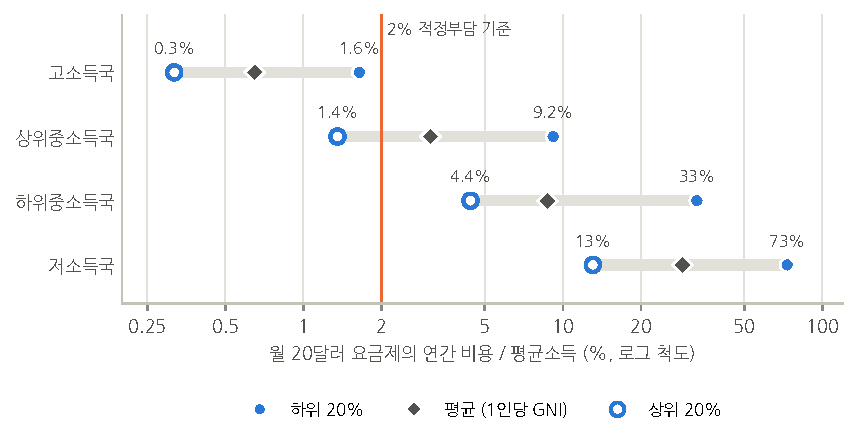
\includegraphics[width=0.92\textwidth]{figures/fig_burden_ko.pdf}
\caption{소득분배 전반에 걸친 20달러 요금제의 부담. 월 20달러 요금제의 연간 비용을 최하위 5분위 평균소득, 인구 전체 평균소득(1인당 GNI), 최상위 5분위 평균소득 대비 비율로 나타내고, 소득집단별로 경제권 중위값을 구했다. 분위 소득은 1인당 GNI에 가계조사 소득점유율을 20\%로 나눈 값을 곱해 근사하였다. 세로선은 광대역 2\% 적정부담 기준이다.}\label{fig:burden}
\end{figure}

분위 평균에서의 부담을 보면 양상이 더 분명해진다(그림~\ref{fig:burden}, 표~\ref{tab:quintile}). 최하위 20\% 가구에게 20달러 요금제의 비용은 중위값으로 고소득국에서 평균소득의 1.6\%이지만 하위중소득국에서 33\%, 저소득국에서 73\%다. 가계조사 자료가 있는 모든 저소득국(19개)과 하위중소득국의 98\%에서는 최상위 20\%에게도 이 요금제가 2\% 기준을 넘으며, 두 집단에서 최상위 분위의 중위 부담은 각각 13\%와 4.4\%다. 따라서 이들 경제에서 업무에 AI를 쓸 가능성이 가장 큰 전문직이 몰려 있는 분배 최상위 가구는 고소득국 최하위 20\% 가구보다 몇 배 큰 부담을 진다.

\begin{table}[t]
\centering
\begin{threeparttable}
\caption{소득 5분위별 20달러 요금제 부담과 모바일 광대역 비교(중위값)}\label{tab:quintile}
\small
\begin{tabular}{@{}lrrrrrr@{}}
\toprule
 & & \multicolumn{3}{c}{20달러 요금제, 분위 평균소득 대비 \%} & 모바일 광대역 & AI 요금제 / \\
\cmidrule(lr){3-5}
소득집단 & $N$ & 하위 20\% & 중위 20\% & 상위 20\% & 2 GB, GNI 대비 \% & 광대역 \\
\midrule
\tabinput{tables/tab_quintile.tex}
\bottomrule
\end{tabular}
\begin{tablenotes}[flushleft]\footnotesize
\item \emph{주:} 분위 점유율은 WDI의 최신 가계조사(중위 조사연도 2021--2023). 모바일 광대역은 월 2 GB 이상의 ITU 데이터 전용 바스켓(선택한 2024년 바스켓)의 월 1인당 GNI 대비 비율이다 \citep{itu2025baskets}. 마지막 열은 20달러를 2024년 광대역 바스켓의 현재 달러 가격으로 나눈 값의 중위값으로, 소득 연도가 서로 다른 부담끼리 나눈 것이 아니다. 광대역 열과 가계조사 열은 각각 이용 가능한 표본을 쓰므로 두 표본이 일치하지 않을 수 있다.
\end{tablenotes}
\end{threeparttable}
\end{table}

\paragraph{기준과 소득 시점에 대한 민감도.} 2\% 기준은 AI를 위해 도출한 것이 아니라 광대역 정책에서 빌려 온 것이므로, 표~\ref{tab:thresholds}에 다른 기준값의 결과를 제시한다. 20달러 기준 가격에서 기준값을 넘는 경제권에 사는 분석 대상 생산가능인구의 비중은 1\%에서 85.6\%, 2\%에서 60.1\%, 5\%에서 44.6\%, 10\%에서 16.7\%다. 2025년 GNI가 있는 182개 경제권으로 한정하면 2\%에서 60.0\%이고, 네 집단의 중위 부담은 0.67\%, 3.09\%, 8.87\%, 28.9\%다. 따라서 이 양상은 오래된 소득 관측치 19개 때문에 생긴 것이 아니다.

\begin{table}[ht]\centering\begin{threeparttable}
\caption{대안 기준을 넘는 경제권과 인구의 비중(20달러 요금제)}\label{tab:thresholds}
\small\begin{tabular}{lrrr}\toprule
기준 & 기준 초과 경제권 & 경제권 비중 & 대상 인구 비중 \\\midrule
\tabinput{tables/tab_thresholds.tex}
\bottomrule\end{tabular}
\begin{tablenotes}[flushleft]\footnotesize\item \emph{주:} 201개 경제권. 인구는 15--64세. 2\% 행은 본문에서 쓰는 광대역 기준이며, 나머지 행은 대안 기준값이다.\end{tablenotes}
\end{threeparttable}\end{table}

\subsection{현지 가격: 사업자는 얼마나 현지화하는가}\label{sec:prices}

사업자가 가난한 시장에서 가격을 낮춘다면 미국 정가로 계산한 부담은 기울기를 과장하게 된다. 이 조사는 관측된 가격표가 부담의 기계적 기울기 $-1$을 얼마나 상쇄하는지 묻는다. 그림~\ref{fig:prices}는 ChatGPT Plus와 ChatGPT Go의 현지 앱스토어 가격을 1인당 소득에 대해 나타내고, 표~\ref{tab:local}은 9개 요금제의 소득집단별 현지 가격 중위값과, 로그 달러 가격을 로그 소득에 회귀해 얻은 기울기 $\hat\beta$를 보여 준다.

\begin{figure}[t]
\centering
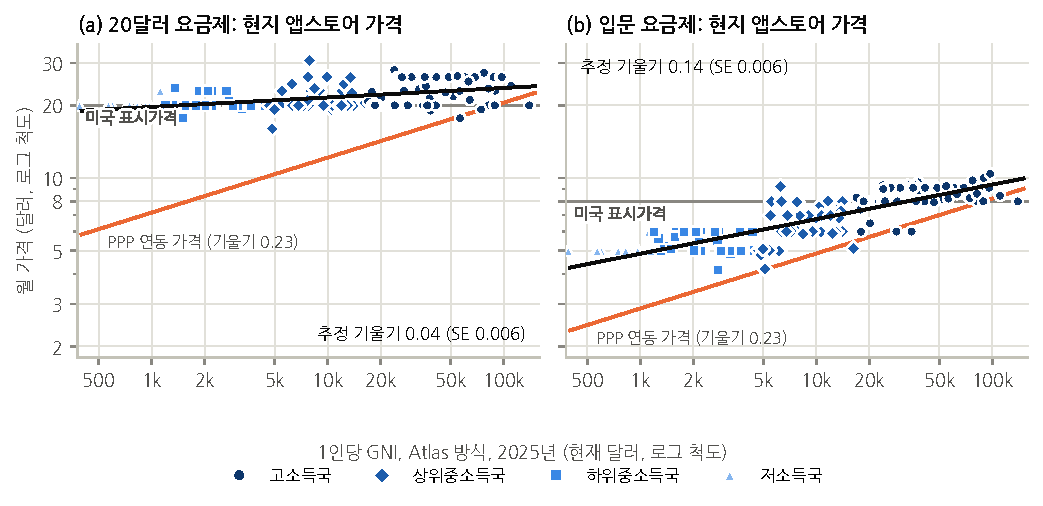
\includegraphics[width=\textwidth]{figures/fig_prices_ko.pdf}
\caption{소득 대비 ChatGPT Plus와 ChatGPT Go의 현지 앱스토어 가격. 국가별 앱스토어의 세금 포함 월 가격을 2026년 9월 27일 시장환율로 달러 환산. 검은 선: 로그-로그 회귀. 주황 선: 미국 가격을 기준으로, 물가수준 대리지표인 Atlas/PPP 소득 비율의 소득 기울기(0.23)를 적용해 현지 물가수준에 연동한 가격. 회색 선: 미국 정가.}\label{fig:prices}
\end{figure}

\begin{table}[t]
\centering
\begin{threeparttable}
\caption{요금제별 현지 가격과 현지화 기울기}\label{tab:local}
\small
\begin{tabular}{@{}lrrrrrrrr@{}}
\toprule
 & 미국 & \multicolumn{4}{c}{현지 가격 중위값(달러)} & \multicolumn{2}{c}{소득 기울기} & \\
\cmidrule(lr){3-6}\cmidrule(lr){7-8}
요금제 & 가격 & 고소득 & 상위중 & 하위중 & 저소득 & $\hat\beta$ & (표준오차) & $N$ \\
\midrule
\tabinput{tables/tab_local.tex}
\bottomrule
\end{tabular}
\begin{tablenotes}[flushleft]\footnotesize
\item \emph{주:} 2026년 9월 27일 앱스토어 월 가격, 미국과 캐나다를 제외하면 세금 포함. $\hat\beta$: $\ln$(현지 달러 가격)을 $\ln$(1인당 GNI)에 회귀한 OLS 기울기, 이분산-강건(HC3) 표준오차. 참고로 로그 물가수준 대리지표(Atlas GNI/PPP GNI)를 로그 소득에 회귀한 기울기는 0.228(표준오차 0.014), GDP 물가수준비율의 기울기는 0.224다. 비례 가격이라면 기울기는 1이다.
\end{tablenotes}
\end{threeparttable}
\end{table}

표준 요금제와 고사용량 요금제의 가격은 거의 균일하다. ChatGPT Plus의 $\hat\beta$는 0.039(표준오차 0.006)이고, Claude Pro와 Google AI Pro의 추정치는 각각 0.026과 0.037이다. ChatGPT Plus의 현지 가격 중위값은 상위중소득·하위중소득·저소득 스토어에서 모두 19.99달러이고, 고소득 스토어의 중위값은 22.99달러로 오히려 더 높다. 앱스토어 가격은 미국과 캐나다 밖에서 부가가치세를 포함하므로, 작은 양의 기울기는 가격차별보다 세금을 반영한 것일 수 있다. 의미 있는 수준으로 현지화된 것은 OpenAI의 입문 요금제뿐이다. ChatGPT Go의 $\hat\beta$는 0.143이며, 네 집단의 중위 가격은 9.05달러, 5.99달러, 5.34달러, 4.99달러이고, 가장 낮은 곳은 인도(4.16달러)와 인도네시아(4.19달러)다. 같은 164개 경제권 표본에서 물가수준 대리지표의 소득 기울기는 0.243이므로, Go의 기울기는 현지 물가수준에 연동할 때의 기울기의 약 60\%이자 비례 가격의 7분의 1이다. Google의 입문 요금제인 AI Plus는 고소득국을 뺀 세 소득집단 모두에서 4.99달러로 일정하다.

$\beta$가 0에 가까우므로 표준 요금제의 부담 탄력성 $\beta-1$은 $-0.96$이다. 현지 가격이 소득 기울기를 거의 전부 부담으로 넘기는 것이다. 표~\ref{tab:store}에서 보듯이 저소득국의 모든 스토어와 하위중소득국 스토어의 86\%가 미국 달러로 가격을 매긴다. 저소득국의 36\%와 하위중소득국의 21\%에는 현지 스토어가 아예 없으므로, 주민은 해외 계정이나 웹으로, 대개 국제 카드를 써서 결제해야 한다. 현지에 표시된 가장 저렴한 유료 요금제는 저소득국 중위 경제에서 4.99달러로 부담이 7.2\%이며, 이 집단의 어느 나라에서도 2\% 기준을 충족하지 못한다. 하위중소득국에서는 38\%에서 충족한다.

\begin{table}[t]
\centering
\begin{threeparttable}
\caption{스토어 이용 가능성, 통화, 현지에 표시된 가장 저렴한 유료 요금제}\label{tab:store}
\footnotesize
\setlength{\tabcolsep}{3pt}
\begin{tabular}{@{}lrrrrrrrr@{}}
\toprule
 & & \multicolumn{3}{c}{ChatGPT 스토어(경제권 \%)} & 달러 & \multicolumn{2}{c}{최저가 유료 요금제} & Plus \\
\cmidrule(lr){3-5}\cmidrule(lr){7-8}
소득집단 & $N$ & 현지 & 없음 & 미제공 & 표시(\%) & 달러 & 부담 & 부담 \\
\midrule
\tabinput{tables/tab_store.tex}
\bottomrule
\end{tabular}
\begin{tablenotes}[flushleft]\footnotesize
\item \emph{주:} ``없음'': 미국 스토어로의 전환(redirect)이 관측됨. ``미제공'': 요청에 대해 앱 페이지가 반환되지 않음. 이는 조사 시점의 수집 결과이며, 서비스 제공 여부를 완전히 판정한 것은 아니다. 최저가 유료 요금제: 현지 스토어의 ChatGPT Go와 Google AI Plus 중 낮은 가격. 부담은 현지 가격 기준 $12p/y\times100$의 중위값.
\end{tablenotes}
\end{threeparttable}
\end{table}

이 양상은 메뉴 설계의 논리와 부합한다. 20달러 요금제를 현지화하면 가치평가가 높은 이용자가 해외 계정으로 차익거래를 할 여지가 생기지만, 역량이 제한된 입문 요금제를 현지화하면 그렇지 않다. 가치평가가 높은 이용자는 스스로 상위 요금제를 고르기 때문이다 \citep{mussa1978monopoly}. 사업자가 국가 간 가격차별을 하는 경우에도 낮춘 품질을 싸게 팔 뿐, 프런티어 요금제의 가격은 거의 현지화하지 않는다. 그렇다면 명제~\ref{prop:margins}에 따라 가격은 현지화되지 않은 채 남아 있는 유료 마진에서 가장 중요해야 한다. 표시가격에는 세금, 플랫폼 규칙, 통화별 가격표도 들어가므로, 이 기울기는 기업의 가격차별 모수가 아니라 가격 메뉴 안의 연관성이다. 또한 이 조사로는 사용 허용량이 적은 요금제가 특정 과업에 충분한지 판단할 수 없다.

\paragraph{강건성: 통화 의존성과 짝지은 요금제 비교.} 같은 통화로 표시된 가격은 환율과 플랫폼 가격표의 충격을 함께 받으며, 통화별 군집의 크기는 매우 불균형하다. Plus 표본에는 달러 표시가 102개, 유로 표시가 25개이고, 나머지 37개는 각각 혼자인 통화다. 따라서 통화별 군집 표준오차는 HC3 표준오차보다 크다(표~\ref{tab:price_revision}). ChatGPT Plus의 군집 95\% 구간은 $[-0.0002, 0.079]$이므로, 이 의존성 가정 아래에서 표준 요금제의 작은 양의 기울기는 0과 구별되지 않으며, 이는 균일성 결과를 오히려 강화한다. Go 기울기의 군집 구간 $[0.114, 0.173]$은 0을 포함하지 않는다. 짝지은 비교는 환율 환산을 아예 제거한다. 각 스토어 안에서 로그 Go/Plus 가격비의 소득 기울기는 0.104(통화 군집 표준오차 0.007, 164개 경제권)이며, 공통 표본에서는 Go와 Plus 기울기의 차이와 정확히 같다. 이 값은 새로운 정보가 아니라 점검 장치다. 이 비율은 두 요금제에 공통인 환율 환산과 비례적 세금을 상쇄하므로, 입문 요금제의 기울기가 환율 환산에서 생긴 착시가 아님을 보여 준다. 기울기는 달러로 표시된 102개 스토어 안에서 0.113, 이들을 빼면 0.112, 달러와 유로 표시를 모두 빼면 0.125다(표~\ref{tab:menu_sensitivity}, 그림~\ref{fig:price_ratio}). 다만 달러 표시를 제외하면 저소득국이 하나도 남지 않으므로, 제외 표본은 중소득·고소득 시장에 관한 결과다. 개별 회귀를 2025년 소득 자료가 있는 경제권으로 한정하면 기울기는 Go 0.149, Plus 0.046이다.

\begin{table}[ht]
\centering\begin{threeparttable}
\caption{표준오차 가정에 따른 가격 기울기}\label{tab:price_revision}
\small\begin{tabular}{lrrrrr}\toprule
요금제 또는 가격비 & 기울기 & HC3 표준오차 & 통화 군집 표준오차 & 군집 95\% 구간 & $N$ \\\midrule
\tabinput{tables/tab_price_revision.tex}
\bottomrule\end{tabular}
\begin{tablenotes}[flushleft]\footnotesize
\item \emph{주:} 모든 결과 변수는 로그. 통화별 군집 CR1 표준오차와 $t_{G-1}$ 구간; 군집 수는 39개(Google AI Pro는 40개). 통화별 군집은 매우 불균형하다(달러 102개, 유로 25개, 단독 통화 37개). 가격비는 같은 스토어에 표시된 두 요금제를 쓴다.
\end{tablenotes}\end{threeparttable}\end{table}

\paragraph{요금제 매칭.} 월 가격은 파싱한 인앱 구매 목록에서 이름과 가격 크기로 고른다(제~\ref{sec:data}절). 이 규칙을 다시 구현하면 ChatGPT Go, ChatGPT Plus, Claude Pro의 모든 스토어-요금제 칸에서 후보 가격이 하나만 남으며, 두 ChatGPT 요금제에서는 연간 가격 제외 기준을 최저 표시가격의 3배, 5배, 8배로 바꾸어도 같은 목록이 선택된다. Google AI Pro에는 후보 가격이 두 개인 칸이 세 개 있으며, 이들을 제외하면 기울기가 0.0370에서 0.0374로 바뀐다. 이 점검은 결과가 특정 선택 규칙에 좌우되지 않음을 보여 준다. 그러나 보관 자료에는 원본 페이지가 아니라 파싱한 기록이 남아 있으므로, 이 점검이 결제 주기 메타데이터나 결제 자격을 확인해 주지는 않는다(제~\ref{sec:limitations}절).

\begin{table}[ht]\centering\begin{threeparttable}
\caption{통화 표본별 Go/Plus 가격비}\label{tab:menu_sensitivity}
\small\begin{tabular}{lrrrr}\toprule
표본 & 기울기 & HC3 표준오차 & HC3 95\% 구간 & $N$ \\\midrule
\tabinput{tables/tab_matched_menu_sensitivity.tex}
\bottomrule\end{tabular}
\begin{tablenotes}[flushleft]\footnotesize
\item \emph{주:} 로그 Go/Plus 표시가격 비율을 로그 Atlas 1인당 GNI에 회귀한 OLS. 구간은 HC3 표준오차와 정규분포 기준을 쓴다. 표본 제한마다 표본이 달라지며, 달러 표시를 제외한 표본에는 저소득국이 남지 않는다.
\end{tablenotes}\end{threeparttable}\end{table}

\begin{figure}[ht]
\centering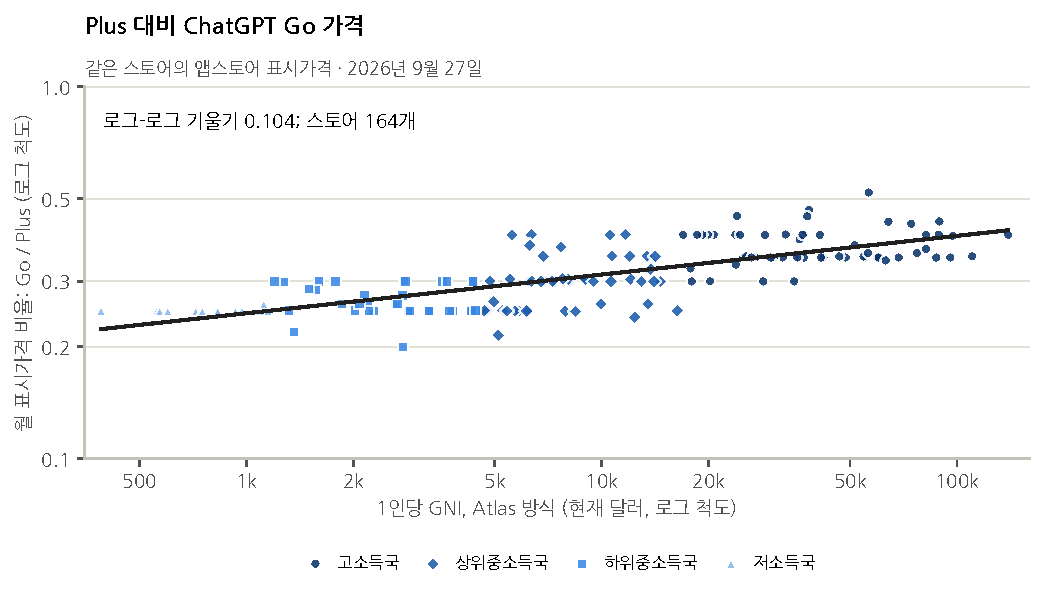
\includegraphics[width=0.85\textwidth]{figures/fig_price_ratio_ko.pdf}
\caption{스토어 안에서의 ChatGPT Go/Plus 가격비. 2026년 9월 27일 같은 스토어에 표시된 두 요금제의 가격을 쓰며, 점 하나가 스토어 하나다. 선은 로그-로그 적합선이다.}\label{fig:price_ratio}
\end{figure}

\subsection{이용 여부: 외연적 마진}\label{sec:extensive}

2026년 2분기 AI 이용자 비중의 중위값은 국가별 추정치가 있는 경제권 기준으로 고소득국 32.3\%, 상위중소득국 18.8\%, 하위중소득국 12.0\%, 저소득국 7.6\%였다(그림~\ref{fig:dynamics}a). 표~\ref{tab:diffusion}은 국가 간 기울기를 보여 준다. 국가별 추정치에서 소득이 로그 1포인트 높으면 이용률은 8.3\%포인트 높고, 탄력성은 0.370(표준오차 0.021, $R^2 = 0.71$)이다. 지역 대체값을 포함하면 탄력성은 0.336으로 낮아지고, 각 묶음을 한 관측치로 합치면 다시 0.367이 된다. 인터넷 이용, 고등교육 등록률, 도시화, 연령구조, 디지털 결제, 지역 고정효과를 통제해도 탄력성은 변하지 않는다(0.355--0.367). 소득을 조건으로 하면 통제변수는 어느 것도 개별적으로 유의하지 않으며, 예외인 부록 표~\ref{tab:controls} 열 (3)--(4)의 도시화($p \approx 0.04$)도 지역 고정효과를 넣으면 유의성을 잃는다.

\begin{table}[t]
\centering
\begin{threeparttable}
\caption{생성형 AI 이용의 소득 기울기(마이크로소프트 AI User Share, 2026년 2분기)}\label{tab:diffusion}
\small
\setlength{\tabcolsep}{5pt}
\begin{tabular}{@{}lrrrrrrr@{}}
\toprule
 & (1) & (2) & (3) & (4) & (5) & (6) & (7) \\
 & 수준(\%p) & \multicolumn{6}{c}{로그 이용자 비중} \\
\cmidrule(lr){3-8}
\midrule
\tabinput{tables/tab_diffusion.tex}
\bottomrule
\end{tabular}
\begin{tablenotes}[flushleft]\footnotesize
\item \emph{주:} OLS, 괄호 안은 HC3 표준오차. 국가별: 국가별 추정치만; 전체: 지역 대체값 포함; 합침: 각 지역 대체 묶음을 인구 가중 로그소득을 가진 한 관측치로 합침. $^\dagger$통제변수(인터넷 이용, 고등교육 등록률, 도시인구 비중, 65세 이상 인구, 온라인 디지털 결제 경험)가 모두 있는 공통 표본. 통제변수 계수는 부록 표~\ref{tab:controls}.
\end{tablenotes}
\end{threeparttable}
\end{table}

기울기의 약 절반은 연결성과 겹친다. 이용하려면 연결이 필요하므로, 이용자 비중은 인터넷 이용률과 인터넷 이용자 대비 AI 이용자 비율의 곱으로 쓸 수 있다. 각 로그 성분을 로그 소득에 회귀하면 탄력성이 정확히 분해되며, 연결성이 0.182, 이 비율이 0.189를 기여하므로 연결성 성분은 기울기의 49\%를 차지한다(부록~\ref{app:connectivity}). 인터넷 이용자 대비 AI 이용자 비율은 상위중소득, 하위중소득, 저소득 집단에서 모두 약 23\%로 고소득국의 37.5\%보다 낮으며, 유료 요금제의 부담이 이 세 집단에 걸쳐 아홉 배로 커지는데도 비고소득국에서 로그 소득에 대한 이 비율의 기울기는 $-0.03$(표준오차 0.06)이다. 이 분해는 인과적 몫이 아니라 회계 항등식이며, 인터넷 이용 시계열은 연령 기준이 다르고 이미 마이크로소프트의 추정량에 들어가 있다. 그렇더라도 외연적 마진에 가격 제약이 구속력을 가진다면 부담이 커질수록 이 비율이 낮아져야 하는데, 세 집단에서는 그렇지 않다. 이 양상은 무료 요금제가 있을 때 명제~\ref{prop:margins}가 예측하는 바와 같지만, 비율이 평평하다는 사실 자체는 모형에서 나오지 않으며 부분적으로는 측정 방식을 반영할 수 있다.

\paragraph{상대적 분산과 절대적 분산의 변화.} 2025년 상반기에서 2026년 2분기 사이 중위 경제의 이용자 비중은 고소득 집단에서 5.5\%포인트, 상위중소득 집단 3.7\%포인트, 하위중소득 집단 2.0\%포인트, 저소득 집단 0.9\%포인트 올랐다(그림~\ref{fig:dynamics}). 상위 세 집단의 비례 성장률은 비슷했고(21--26\%), 뒤처진 경제는 로그로는 약간 더 빨리 성장했다. 로그 성장률을 초기 로그 비중에 회귀하면 계수는 $-0.026$(표준오차 0.011)이고, 로그 비중의 국가 간 표준편차는 0.564에서 0.553으로 줄었다. 퍼센트포인트로는 정반대다. 소득이 로그 1포인트 높을수록 증가폭이 1.37\%포인트 크고(표준오차 0.13), 표준편차는 10.9\%포인트에서 12.8\%포인트로 커졌으며, 고소득국과 하위중소득국 중위 경제의 격차는 16.3\%포인트에서 20.3\%포인트로 벌어졌다. 이 결과는 소득이 낮은 나라들에서 비례 성장이 더 빠르다는 보고 \citep{chatterji2025how}와 격차가 벌어지고 있다는 보고 \citep{microsoft2026h2,liu2025who}를 조화시킨다. 두 보고는 확산 초기 곡선을 서로 다르게 읽은 것이다. 다만 사업자가 추정한 네 시점만으로는 곡선의 모양을 확정할 수 없고, 초기 수준의 측정오차는 성장률을 초기 수준에 회귀하는 분석에도 영향을 준다.

\begin{figure}[t]
\centering
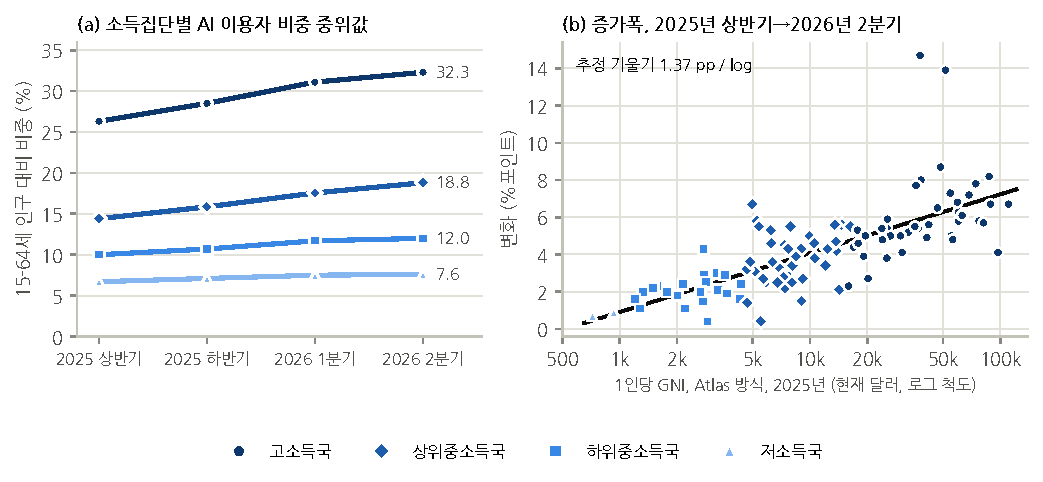
\includegraphics[width=\textwidth]{figures/fig_dynamics_ko.pdf}
\caption{확산의 동학. (a) 소득집단별 AI 이용자 비중 중위값, 마이크로소프트 국가별 추정치(저소득국: 세 경제권). (b) 2025년 상반기와 2026년 2분기 사이 AI 이용자 비중 변화와 1인당 GNI, 로그-선형 적합 기울기.}\label{fig:dynamics}
\end{figure}

\subsection{1인당 Claude 이용량: 유료 마진의 불완전한 창}\label{sec:twomargins}

Anthropic의 자체 보고서는 생산가능인구 1인당 GDP를 써서 Claude 이용량의 소득 기울기가 0.7 가까이 된다고 보고했다 \citep{appel2025uneven}. 여기서의 기여는 그 기울기 자체가 아니라, 공통 표본에서 다른 공개 지표와 비교한 것이다.

그림~\ref{fig:twomargins}는 두 지표가 모두 있는 96개 경제권에서 각 지표의 국가 간 평균 대비 로그 편차를 소득에 대해 나타낸다. 이 표본은 고소득국 42개, 상위중소득국 33개, 하위중소득국 20개, 저소득국 1개(르완다)로 이루어져 있다. 따라서 이 비교는 하위중소득국에서 고소득국에 이르는 기울기를 보여 줄 뿐, 저소득국에 관해서는 말해 주는 바가 적다. 1인당 Claude 이용량은 소득에 따라 두 배 가파르게 오른다. 그 탄력성은 0.711(표준오차 0.036)로 이용 여부의 0.371(표준오차 0.026)보다 크며, 둘의 차이는 0.340(군집 표준오차 0.034, 부트스트랩 95\% 구간 0.27--0.40)이다. 표~\ref{tab:twomargins}는 이 격차가 함수 형태나 표본에서 생긴 것이 아님을 보여 준다. 상한 효과를 고려해 이용자 비중을 로그오즈로 표현해도(0.50 대 0.71), 고소득국을 제외해도(0.33 대 0.69), 인터넷 이용·고등교육 등록률·도시화를 통제해도(0.31 대 0.55), 이전 측정 시점에서도(0.38 대 0.62), 지역 대체값을 포함해도(0.36 대 0.73) 격차는 유지된다.

\begin{figure}[t]
\centering
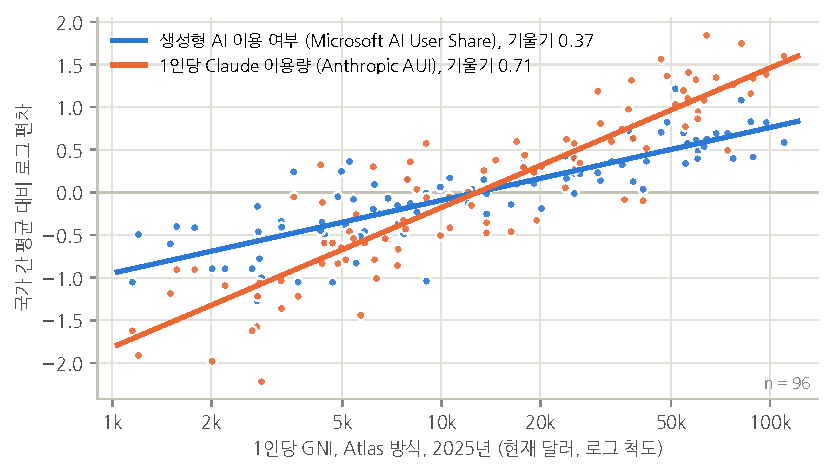
\includegraphics[width=0.9\textwidth]{figures/fig_two_margins_ko.pdf}
\caption{AI 확산의 두 마진. 두 지표가 모두 있는 96개 경제권에서 마이크로소프트 AI User Share(생성형 AI 이용 여부, 2026년 2분기, 국가별 추정치)와 Anthropic AUI(1인당 Claude 이용량, 2026년 5월)의 국가 간 평균 대비 로그 편차와 1인당 GNI. 선은 OLS 적합이며 기울기는 소득탄력성이다.}\label{fig:twomargins}
\end{figure}

\begin{table}[t]
\centering
\begin{threeparttable}
\caption{이용 여부와 1인당 Claude 이용량의 소득탄력성}\label{tab:twomargins}
\small
\setlength{\tabcolsep}{5pt}
\begin{tabular}{@{}>{\raggedright\arraybackslash}p{7.6cm}ccr@{}}
\toprule
추정 방식 & 이용 여부(MS) & Claude 이용량(AUI) & $N$ \\
\midrule
\tabinput{tables/tab_twomargins.tex}
\bottomrule
\end{tabular}
\begin{tablenotes}[flushleft]\footnotesize
\item \emph{주:} 각 칸은 공통 표본에서 로그 1인당 GNI에 대한 OLS 기울기이며, 결과 변수는 로그다. 다만 따로 표시한 마이크로소프트 로그오즈 행은 같은 탄력성이 아니다. 괄호 안은 HC3 표준오차이며, 쌓아 추정한 차이 행만 예외다. MS: 마이크로소프트 AI User Share; AUI: Anthropic AI Usage Index. 차이 검정은 두 결과 변수를 쌓고 결과 변수별 절편과 기울기를 두며 경제권 단위로 군집화하였다. 부트스트랩은 경제권을 2,000회 재추출하였다. 주 표본은 고소득국 42개, 상위중소득국 33개, 하위중소득국 20개, 저소득국 1개이며, 고소득국을 제외하면 54개다.
\end{tablenotes}
\end{threeparttable}
\end{table}

측정된 기울기도 연속적이지는 않지만 더 가팔라졌다. 다섯 시점 모두 관측된 111개 경제권에서 탄력성은 2025년 8월과 11월 0.68, 2026년 2월 0.74, 4월 0.77, 5월 0.73이었다. 2025년 8월에서 2026년 2월까지의 증가(0.064, 군집 표준오차 0.018)는 유의하지만, 2026년 2월에서 5월까지의 변화($-0.006$, 표준오차 0.016)는 유의하지 않다. 이 기간에 Anthropic의 릴리스는 달라졌다. 이후 릴리스에 Cowork 세션과 월 단위 측정 기간이 추가되었으므로, 이 시계열은 엄밀히 같은 대상을 추적한 것이 아니라 측정된 Claude 이용량을 나타낸다. 시점마다 Anthropic의 기준을 충족한 경제권 전체로 추정해도 결과는 비슷하며(부록 표~\ref{tab:auitime}), 기울기가 가팔라진 것은 채택이 낮은 나라들이 조금 더 뒤처졌다는 Anthropic 자체의 발견과도 일치한다 \citep{massenkoff2026learning}. 이용의 구성도 다르다. Claude 대화 중 학업(coursework)의 비중은 소득이 로그 1포인트 높을수록 4.7\%포인트 낮아, 저소득국 중위 경제의 35\%(다섯 경제권)에서 고소득국 중위 경제의 17\%로 내려간다. 이 기울기는 소득이 낮은 지역에서 학습이 AI의 주요 진입 경로 가운데 하나라는 증거 \citep{microsoft2026q2,daepp2026how}와도, 학업 용도가 무료 이용에 더 적합할 수 있다는 Anthropic의 관찰 \citep{appel2026primitives}과도 부합한다. 세 번째 출처인 Google의 Gemini 1인당 채택 5분위도 소득과 양의 관계를 보이지만 그 관계는 덜 긴밀하다(195개 경제권, 스피어먼 상관 0.46). 다만 순위 척도이고 제품 범위도 달라 탄력성을 직접 비교할 수는 없다.

\paragraph{기울기 차이의 직접 추정.} 공통 표본에서 두 로그소득 기울기의 차이는 $\ln(AUI_c/D_c)$를 로그 소득에 회귀한 기울기와 같으며, 두 회귀에 같은 통제변수를 넣어도 마찬가지다. 기준 차이는 0.340(HC3 표준오차 0.034)이며, 2025년 GNI만 쓰면 0.356, 지역 고정효과를 넣으면 0.266, 인터넷·교육·도시화를 통제하면 0.232다(표~\ref{tab:gap_revision}). 국가를 하나씩 빼면 0.329--0.351이고, 생산가능인구로 가중하면 0.476인데, 이는 큰 나라들이 좌우하는 다른 추정 대상이다. 이 계산들 가운데 어느 것도 식~\eqref{eq:aui_identity}의 사업자 점유율 성분과 이용자당 대화 수 성분을 분리하지 않는다.

\begin{table}[ht]\centering\begin{threeparttable}
\caption{두 소득탄력성 차이의 민감도}\label{tab:gap_revision}
\small\begin{tabular}{lrrrr}\toprule
추정 방식 & 차이 & HC3 표준오차 & 95\% 구간 & $N$ \\\midrule
\tabinput{tables/tab_gap_revision.tex}
\bottomrule\end{tabular}
\begin{tablenotes}[flushleft]\footnotesize\item \emph{주:} 종속변수는 $\ln(AUI/D)$이며, 기준은 공통 경제권 96개를 쓴다. 구간은 정규 근사를 쓴다. 인구 가중은 추정 대상을 바꾼다.\end{tablenotes}
\end{threeparttable}\end{table}

이러한 양상은 유료 장벽이 무료 장벽보다 높고 현지화가 약할 때(20달러 요금제에서 $\hat\beta \approx 0.04$) 명제~\ref{prop:margins}가 예측하는 바다. 그러나 유료 가입이 관측되지 않으므로 이는 명제의 검정이 아니다. 사업자 선택, 대화 빈도, 제품 범위, 업무 구성, 지표마다 다른 측정오차도 같은 기울기 순서를 만들어 낼 수 있으며, Anthropic 릴리스의 포괄 범위가 바뀌었으므로 기울기가 가팔라진 것도 행동의 발산을 깨끗하게 추정한 종단 결과가 아니다. 제~\ref{sec:discussion}절에서 이 대안들을 따져 본다.

% ================================================================================================
\section{논의}\label{sec:discussion}

\subsection{증거가 보여 주는 것과 보여 주지 못하는 것}

증거는 세 가지 진술을 뒷받침한다. 첫째, 표준 요금제의 표시가격은 나라마다 거의 같으며, 의미 있는 현지화는 품질을 낮춘 입문 요금제에서만 나타난다. 둘째, 그 결과 균일한 달러 가격은 소득집단 사이에 약 45배 다른 부담을 지우며, 이 기울기는 대안 분모, 대안 기준, 소득 시점을 바꾸어도 유지된다. 셋째, 두 공개 이용 지표는 소득 기울기가 서로 다르다. 이용 여부는 소득에 따라 중간 정도로 기울어 있고, 그 기울기의 절반가량은 연결성과 겹치며, 유료 요금제의 부담이 커져도 인터넷 이용자 대비 AI 이용자 비율은 낮아지지 않는다. 반면 1인당 Claude 이용량은 소득에 따라 두 배 가파르게 기울어 있고, 2025년 말에서 2026년 초 사이에 더 가팔라졌다.

그러나 이 증거는 가격이 더 가파른 Claude 기울기의 원인임을 입증하지 않는다. 제~\ref{sec:mechanism}절의 무료 요금제 모형은 관측된 순서를 예측하지만, 여러 대안도 같은 순서를 예측할 수 있다. 언어: 프런티어 AI 비서는 자원이 풍부한 언어에서 가장 잘 작동하며, 현지 언어 지원이 약한 곳에서는 영어 대화가 과대 대표된다 \citep{daepp2026how}. 제품과 브랜드: AI 이용자 가운데 Claude의 비중은 인지도, 직업, 경쟁 제품에 따라 달라질 수 있으며, 소득이 낮은 많은 시장에서 Claude는 ChatGPT, Gemini, 메타의 AI 비서보다 덜 알려져 있다. 업무 구성: Claude 이용은 소프트웨어와 전문직 과업에 치우쳐 있고, 이들 과업의 고용 비중은 소득과 함께 커진다 \citep{gmyrek2025generative}. 측정: 마이크로소프트 추정량은 잡음이 큰 나라의 값을 세계 평균 쪽으로 수축하고 기기 보정계수에 하한을 두어 국가 간 변동을 압축한다. Anthropic의 공표 기준은 대화량으로 나라를 선택하며, 이 지수는 무료와 유료 계정을 합산하므로 이용자당 대화 수는 요금제 상태보다 업무 관행을 반영할 수 있다. 고소득국을 제외하거나 교육을 통제해도 격차가 유지되므로 강건성 점검은 이러한 우려의 일부를 다룬다. 그러나 가격 효과에 이르는 믿을 만한 유일한 경로는 소득의 함수가 아닌 가격 변동이다.

\subsection{실행 가능한 평가 과제}

이제 그러한 변동이 생겼다. ChatGPT Go는 인도에 이어 170개국에 단계적으로 출시되었고 \citep{openai2026go}, Google은 2025--2026년에 AI Plus와 AI Ultra를 도입하고 가격을 조정했다 \citep{google2026io}. OpenAI는 2026년 9월 Pro 요금제의 사용 허용량과 가입 자격을 바꾸었고(제~\ref{sec:tariff}절), 여러 시장에서 이동통신 가입과 결합한 한시적 프리미엄 요금제가 등장했으며, 앱스토어 가격표는 환율과 세금에 따라 바뀐다. 이러한 사건을 분기별 마이크로소프트 시계열, 월별 Anthropic 시계열과 결합하면, 현지화된 요금제가 도입되기 전후의 경제를 비교하는 이중차분·사건연구 설계가 가능하다.

요구 조건은 까다롭다. 결과는 개입이 일어나는 수준에서 측정해야 한다. 곧 해당 사업자와 요금제의 실효 가격, 유료 전환, 활성 이용자, 이용자당 이용량, 해지를 안정된 인구 기준과 제품 범위에서 측정해야 한다. 요금제 도입 시점은 시장 성장에 반응할 수 있고 마케팅, 결합상품, 모델 개선과 겹칠 수 있으므로, 사건연구에는 충분한 처치 전 관측치, 그럴듯한 비교집단, 예상 효과와 파급 효과에 대한 점검, 출시 코호트마다 다른 효과를 허용하는 추정량이 필요하다 \citep{callaway2021did}. ChatGPT 가격 변화에 대한 Claude 이용의 반응은 사업자 간 교차 효과를 측정할 뿐, 유료 채택에 대한 ChatGPT의 자기가격탄력성을 측정하지 않는다. 통화나 세금의 변화는 소득과 다른 구매에도 영향을 주므로 자동으로 타당한 도구변수가 되지도 않는다. 무료 요금제로의 대체와 고용주 제공 접근을 따로 기록하면서 무작위 할인이나 기관 접근을 제공하는 실험이 가입 효과를 가장 깨끗하게 식별할 것이다. 사업자가 국가별 유료 구독자 수와 실효 가격을 공개한다면 이 모든 설계가 훨씬 정밀해질 수 있다.

\subsection{정책적 함의}

이 결과는 네 가지 정책 문제와 관련되며, 아래에서는 관련된 마진 순서로 제시한다.

\emph{외연적 마진의 전제조건인 연결성.} 연결, 기기, 전력은 모든 이용의 전제조건이며, 이용 기울기의 절반은 연결성의 기울기와 겹친다. 고소득국 아래 집단에서 인터넷 이용자 대비 AI 이용자 비율이 평평하다는 사실은, 연결된 사람들이 AI를 쓸지 말지를 제약하는 요인이 가격보다 접근과 보완재라는 견해 \citep{worldbank2026wdr,itu2025ff}와 부합하지만, 그 견해를 입증하지는 않는다. 컴퓨팅과 데이터 인프라는 그 위의 또 다른 층이다 \citep{lehdonvirta2024compute}. 아프리카에 고속 인터넷이 들어온 사례는 이러한 투자가 그 자체로 고용과 생산성을 높인다는 점을 시사한다 \citep{hjort2019arrival}.

\emph{유료 마진을 위해서는 품질을 낮춘 요금제만이 아니라 프런티어 접근을 현지화해야 한다.} 3급 가격차별의 후생 효과는 일반적으로 모호하지만, 균일 가격이라면 열리지 않았을 시장을 여는 경우에는 긍정적인 경향이 있다 \citep{varian1985price,aguirre2010monopoly}. 정가가 평균소득의 4분의 1을 넘는 프런티어 요금제가 그러한 경우일 수 있다. 현지 통화 스토어, 통신사 결제, 현지 물가에 연동한 가격의 기간 제한·사용량 제한 프런티어 접근은 실행 가능한 방안이다. 20달러 요금제의 가격을 균일하게 묶어 두는 차익거래 위험은 프런티어 모델 제공을 막지 않고도 사용량 한도로 억제할 수 있다. 사용 허용량이 적은 요금제가 특정 과업에 충분한지는 이 조사로 판단할 수 없다.

\emph{기관을 통한 접근.} AI의 생산성 효과에 관한 증거는 거의 모두 개인 구독이 아니라 고용주가 제공한 도구에서 나온다 \citep{brynjolfsson2025generative,cui2024effects}. 학교, 대학, 공공기관, 고용주는 접근을 가계소득과 분리할 수 있다. 세계은행이 나이지리아에서 수행한 실험에서는 감독하에 운영한 GPT-4 튜터링 프로그램이 상당한 학습 효과를 냈다 \citep{desimone2025chalkboards}. 새로운 보건 제품에 대한 보조금 연구는 무료 체험이 장기 채택을 밀어내기보다 학습을 거쳐 늘릴 수 있음을 시사하며 \citep{dupas2014short}, 작은 가격조차 빈곤층의 이용을 크게 줄일 수 있다 \citep{cohen2010free}.

\emph{투명성.} 국가별 유료 구독, 실효 가격, 사용 한도에 관한 공개 자료가 없다는 점이 AI 접근 연구를 제약한다. 날짜가 명시된 국가별 가격, 세금, 지원 결제수단, 요금제 한도, 제품 정의를 기계가독 형태로 공개하고, 무료와 유료 계정, 이용자 수와 이용자당 이용량을 구분한 이용 통계를 공개한다면 위의 설계를 실행할 수 있다. 부록~\ref{app:protocol}에 이러한 기록에 담겨야 할 항목을 정리하였다.

\subsection{한계}\label{sec:limitations}

첫째, 부담은 지출이 아니라 정규화된 가격이며, 분위 소득은 소득과 소비 개념이 섞인 가계조사 점유율에 기초한 근사다. 전국 평균 기준 비율이 높은 경제에 사는 사람이라고 해서 반드시 구독료를 감당할 수 없는 것은 아니다. 둘째, 앱스토어 조사는 하나의 경로에서 하루 동안의 표시가격을 관측한다. 표시가격은 웹 가격이나 실제 결제 금액과 다를 수 있고, 회귀에서 분리하지 않은 플랫폼 수수료와 세금을 포함한다. 또 보관 자료에는 원본 페이지가 아니라 파싱한 목록 기록이 남아 있으므로, 각 목록의 월 결제 주기는 상품 메타데이터로 확인한 것이 아니라 이름과 가격 크기로 추론한 것이다. 판촉과 결합상품은 반영되지 않는다. 셋째, 마이크로소프트 시계열은 데스크톱 원격측정에 기초한 모형 추정치이며, 대부분의 저소득국에는 국가별 값이 없다. 이 집단에 관한 결과는 세 경제권이나 지역 대체 묶음에 의존하며, 두 지표의 비교에는 저소득국이 하나뿐이다. 넷째, Anthropic 지수는 한 사업자의 소비자 제품만 포괄하고 유료와 무료 이용자를 구분하지 않으므로 유료 마진을 불완전하게 대리하며, 그 포괄 범위는 릴리스마다 바뀌었다. 다섯째, 모든 회귀는 횡단면적이고 기술(記述)적이며, 그 표준오차는 사업자 추정량 내부의 불확실성을 반영하지 않는다. 여섯째, 분석 틀은 선호, 분산, 과업 가치를 고정하고, 경쟁 사업자, 고용주 제공 접근, 후생을 생략하며, 이용 지표에 맞추어 보정되지 않았다. 수렴 계산은 과업 노출도와 과업 내 채택률의 대리변수로 직업 노출도와 인구 전체의 이용률을 쓴다.

% ================================================================================================
\section{결론}\label{sec:conclusion}

생성형 AI는 세계 상품처럼 가격이 매겨지지만 지역 상품처럼 경험된다. 표준 20달러 요금제는 어디서나 거의 같은 가격으로 표시되므로, 그 비용은 부유한 나라의 중위값에서는 평균소득의 1\% 미만이지만 가난한 나라의 중위값에서는 4분의 1을 넘는다. 이 요금제는 세계 생산가능인구 대부분에게 광대역 적정부담 기준을 넘으며, 저소득국에서는 최상위 20\%에게도 마찬가지다. 부분적으로라도 현지화된 것은 OpenAI의 입문 요금제뿐이며, 그 현지화 정도는 현지 물가수준에 연동할 때의 약 60\%에 그친다.

공개 이용 자료는 무료 요금제가 AI를 쓸지 말지의 결정에서 가격을 걷어 냈다는 해석과 부합한다. 이 마진에서 소득 기울기의 절반가량은 연결성과 겹치며, 유료 요금제의 부담이 커져도 인터넷 이용자 대비 AI 이용자 비율은 낮아지지 않는다. 반면 사람들이 프런티어 역량을 얼마나 쓰는지는 여전히 소득에 묶여 있다. 1인당 Claude 이용량의 기울기는 두 배 가파르며, 2025년 8월에서 2026년 2월 사이에 더 가팔라졌다. 프런티어 이용을 소득에 묶어 두는 것이 언어, 제품의 도달 범위, 업무 구성이 아니라 가격인지는 국가 간 자료로 말할 수 없다. 현지화된 요금제의 단계적 출시와 최근의 사용 허용량 변경 덕분에, 가격과 이용 권리와 유료 이용을 그것이 바뀌는 수준에서 기록한다면 이제 이 질문에 답할 수 있다.

AI가 경험이 적은 근로자를 가장 많이 돕는다는 조건부 증거는 사실이다. 그러나 접근과 노출도가 함께 따라가지 않으면 조건부 평등화는 수렴으로 합쳐지지 않으며, 현재 수치로 보면 접근과 노출도는 따라가지 못하고 있다. 앞으로 따라갈지는 모델이 얼마나 유능해지느냐보다, 누가 프런티어 모델에 접근하거나 그 비용을 감당할 수 있고, 얼마나 많이 쓸 수 있으며, 출시 후 얼마나 빨리 쓸 수 있는지에 더 달려 있다.

% ================================================================================================
\section*{선언}
\paragraph{생성형 AI 및 AI 보조 기술 사용 선언.} 저자는 이 연구를 준비하는 과정에서 문헌 탐색, 코드 작성과 자료 처리, 원고 작성과 번역, 그리고 방법론과 재현성 패키지 점검에 ChatGPT와 Codex(OpenAI), Claude(Anthropic)를 활용하였다. 이 도구를 사용한 뒤 저자는 필요에 따라 내용을 검토·수정하였으며 출판물의 내용에 전적인 책임을 진다.
\paragraph{자료 이용 가능성.} 모든 자료는 공개되어 있다. 재현성 패키지(원자료 추출본, 코드, 산출물)는 Zenodo에 보관되어 있다: \href{https://doi.org/10.5281/zenodo.23006365}{https://doi.org/10.5281/zenodo.23006365}(전체 버전; 버전 2.0은 이 원고의 영문판에, 버전 1.8은 이전 워킹페이퍼에 대응한다). 부록~\ref{app:data}에서 패키지 내용을 설명한다.
\paragraph{연구비와 이해관계.} 이 연구는 특정 연구비를 받지 않았으며, 저자는 이해관계가 없음을 밝힌다.

\bibliographystyle{apalike-doi}
\bibliography{references}

% ================================================================================================
\appendix
\section{무료·유료 접근에 관한 조건부 분석 틀}\label{app:tiermodel}
\label{sec:conditional_access}

연결된 개인이 비이용, 무료 요금제, 유료 요금제 가운데 하나를 고른다고 하자. $v>0$는 실효 AI 서비스 한 단위에 대한 개인의 월 화폐 가치평가다. 예컨대 $v=\theta w$일 수 있으며, 여기서 $w$는 월 소득, $\theta$는 개인의 활동에서 AI가 갖는 관련성이다. $0<q_F<q_P$는 두 요금제의 서비스 수준, $p_c>0$는 월 유료 가격, $\tau>0$는 두 요금제에 공통인 시간, 학습, 그 밖의 참여 비용을 월 화폐액으로 환산한 값이다. 효용은 다음과 같다.
\begin{equation}
 u_0=0,\qquad u_F=vq_F-\tau,\qquad u_P=vq_P-\tau-p_c.
 \label{eq:tier_utilities}
\end{equation}
이 서비스 수준은 이론적 대상이며, 특정 모델, 관측된 구독 상품명, 측정된 기술 프런티어와 대응할 필요가 없다. 이 틀은 경쟁 공급자, 고용주 제공 접근, 공유, 이용량에 따라 달라지는 참여 비용을 생략한다.

$\Delta q=q_P-q_F$라 하자. 세 선택지를 모두 직접 비교하면 이용 여부와 유료 이용의 문턱은 다음과 같다.
\begin{equation}
 T_{D,c}=\min\left\{\frac{\tau}{q_F},\frac{\tau+p_c}{q_P}\right\},
 \qquad
 T_{P,c}=\max\left\{\frac{p_c}{\Delta q},\frac{\tau+p_c}{q_P}\right\}.
 \label{eq:general_thresholds}
\end{equation}
따라서 무료 선택지가 있다는 것만으로 총 채택이 유료 가격과 무관해지지는 않는다. 유료 선택지가 충분히 매력적이면 비이용자를 곧바로 끌어올 수 있다.

$\kappa_c$를 참여에 필요한 연결성과 보완 자원을 갖춘 인구의 비중이라 하자. 이 집단에 속한다는 조건에서
\begin{equation}
 \ln v\sim N(\mu_c,s^2),\qquad
 \mu_c=\mu_0+\ln(y_c/y_0),\qquad s>0
 \label{eq:conditional_distribution}
\end{equation}
를 가정한다. 여기서 $y_c$는 국가 소득 지수, $y_0$는 기준값이다. 이 위치 이동 가정은 양식화이며, 국민 GNI를 가계소득이나 AI 활용의 수익과 연결하는 항등식이 아니다. 분포를 참여 자격을 조건으로 정의하면 $\kappa_c$를 곱하는 과정이 명시적으로 드러난다. 같은 분포를 조건 없이 적용하려면 추가적인 선택 가정이 필요하다. 서비스 수준, 참여 비용, 분산이 공통이라면 어떤 요금제든 쓰는 인구 비중과 유료 요금제를 쓰는 인구 비중은 다음과 같다.
\begin{equation}
 D_c=\kappa_c\Phi\left(\frac{\mu_c-\ln T_{D,c}}{s}\right),\qquad
 P_c=\kappa_c\Phi\left(\frac{\mu_c-\ln T_{P,c}}{s}\right).
 \label{eq:general_shares}
\end{equation}
공통 $\tau$ 가정은 실질적인 가정이다. 참여 비용이 $\tau_c\propto y_c^\lambda$로 달라진다면, 무료 서비스 수준이 고정되어 있더라도 중첩 체제의 채택 기울기는 $\varepsilon_\kappa+(1-\lambda)h(z_D)/s$가 된다. 시간 비용의 화폐 가치는 임금과 함께 오를 수 있으므로, 기본 가정은 경제적으로 의미 있는 기울기 변동의 원천 하나를 배제한다. 참여 비용의 임의적인 이질성은 두 문턱 공식과 공통 유료 가격을 유지하면서 일반적으로 $v$에 흡수될 수 없다.

\paragraph{문턱의 순서.}
다음이 성립하면
\begin{equation}
 \frac{p_c}{\Delta q}>\frac{\tau}{q_F},
 \label{eq:nested_condition}
\end{equation}
$T_{D,c}=\tau/q_F$, $T_{P,c}=p_c/\Delta q$이다.
이 체제에서는 $\kappa_c$, 서비스 수준, 참여 비용이 변하지 않는 한 유료 가격이 조금 바뀌어도 $D_c$는 변하지 않는다. 부등호가 반대이면 두 문턱은 모두 $(\tau+p_c)/q_P$가 되고, 유료 가격은 유료 이용뿐 아니라 이용 여부에도 영향을 준다.

\paragraph{증명.}
무료 요금제는 $v\geq\tau/q_F$일 때 비이용보다 낫다. 유료 요금제는 $v\geq(\tau+p_c)/q_P$일 때 비이용보다, $v\geq p_c/\Delta q$일 때 무료 요금제보다 낫다. 이 비교들로 식~\eqref{eq:general_thresholds}가 성립한다. 조건~\eqref{eq:nested_condition} 아래에서 세 문턱은 $\tau/q_F<(\tau+p_c)/q_P<p_c/\Delta q$의 순서를 가진다. 조건이 반대이면 이 순서도 반대가 되므로 두 체제가 모두 성립한다. 등호에서는 문턱들이 일치한다.
\qed

\begin{proposition}[국지적 소득 기울기]\label{prop:margins}
엄격한 중첩 문턱 체제에서
$z_D=(\mu_c-\ln(\tau/q_F))/s$,
$z_P=(\mu_c-\ln(p_c/\Delta q))/s$,
$h(z)=\phi(z)/\Phi(z)$,
$\beta=\partial\ln p_c/\partial\ln y_c$,
$\varepsilon_\kappa=\partial\ln\kappa_c/\partial\ln y_c$로 정의하자.
그러면
\begin{equation}
 \varepsilon_D=\varepsilon_\kappa+\frac{h(z_D)}{s},\qquad
 \varepsilon_P=\varepsilon_\kappa+(1-\beta)\frac{h(z_P)}{s}
 \label{eq:income_gradients}
\end{equation}
이다. 균일 가격이면 $\varepsilon_P>\varepsilon_D$다. 현지 가격 수준과 그에 따른 문턱 값을 고정할 때, $\beta<\beta^*\equiv1-h(z_D)/h(z_P)$이면 이 순서가 유지되며, 여기서 $0<\beta^*<1$이다.\end{proposition}

\paragraph{증명.}
$\partial\mu_c/\partial\ln y_c=1$이므로 식~\eqref{eq:general_shares}의 로그를 미분하면 식~\eqref{eq:income_gradients}를 얻는다. 엄격한 문턱 순서에서 $z_P<z_D$다. 아래 꼬리 역밀스비 $h$는 순감소 함수이므로 $h(z_P)>h(z_D)$다. 두 탄력성의 차를 구해 같아지는 점을 풀면 $\beta^*$를 얻는다. \qed

$\beta$에 걸친 비교는 국지적이다. 한 가지 구현은 가격표 $p_\beta(y)=p_0(y/y_0)^\beta$들을 공통 기준점 $y_0$에서 비교하는 것이다. 그 기준점을 벗어나면 가격표를 바꾸는 것이 유료 문턱도 움직이므로, 이 명제는 현지화 정책의 전역적 효과를 입증하지 않는다. 후생 효과도 입증하지 않는다. 이 명제의 실질적 함의는 조건부다. 문턱이 중첩되고 분포에 관한 가정이 유지된다면, 무료 요금제는 최초 채택의 결정 요인을 유료 전환의 결정 요인과 분리할 수 있다.

문턱이 뒤바뀐 체제에서는 같은 계산이 대신 다음을 준다.
\begin{equation}
 \varepsilon_D=\varepsilon_P
 =\varepsilon_\kappa+
 \left(1-\beta\frac{p_c}{\tau+p_c}\right)\frac{h(z)}{s},
 \qquad z=\frac{\mu_c-\ln((\tau+p_c)/q_P)}{s}.
 \label{eq:reversed_gradients}
\end{equation}
이때에는 무료 요금제가 개인의 최적 선택이 되는 구간이 없다. 이 극단적 경우는 무료 제품이 실제로 존재한다는 사실만으로 가격 독립성을 입증할 수 없는 이유를 분명히 보여 준다. 더 일반적으로, 언어 지원, 시간 비용, 서비스 품질, 인터넷 연결 여부의 (자기)선택, 가치평가의 분산이 나라마다 다르면 기울기에 추가 항이 생긴다. 이러한 가능성은 실질적으로 중요하며 소득 회귀로 배제되지 않는다. 따라서 이 틀은 이러한 경쟁 설명들을 열어 둔 채 접근에 관한 질문을 정리하는 데 쓰여야 한다.


\section{자료 구축과 재현}\label{app:data}

\paragraph{재현성 패키지.} 패키지에는 원자료 추출본(세계은행 API 추출본, 커밋 507c316 시점의 마이크로소프트 자료, Anthropic Economic Index 파일, Google ATLAS 자료, ITU 요금 바스켓, 앱스토어 수집 자료, 환율), 처리 스크립트, 분석, 그림과 표 생성 코드가 들어 있으며, README는 사회과학 데이터 편집자(Social Science Data Editors)의 템플릿을 따른다. 본문의 모든 수치는 이 패키지로 재현할 수 있다. 대부분은 분석 스크립트가 \nolinkurl{output/results.json}에 기록하고, 민감도 분석은 \nolinkurl{revision_audit/}와 \nolinkurl{publication_upgrade/}의 스크립트가 기록하며, 나머지는 그 값에서 바로 계산되거나 출력 표, 가공 자료, 스크립트에서 읽을 수 있다. 함께 제공한 원자료 추출본에서 파이프라인을 다시 실행하면 결과 파일의 865개 항목과 모든 표 본문이 바이트 단위까지 그대로 재현되며, 핵심 회귀를 NumPy로 독립적으로 구현한 결과도 보고된 추정치와 일치한다. 고정한 마이크로소프트 원천 자료, Anthropic의 네 릴리스, ITU 통합문서도 다시 내려받아 처리했으며, 파생 파일은 패키지에 든 것과 바이트 단위로 같았다. 패키지로 할 수 없는 것은 앱스토어 추출 자체를 다시 실행하는 일이다. 패키지에는 원본 페이지가 아니라 파싱한 목록 기록이 들어 있기 때문이다. 제~\ref{sec:prices}절의 요금제 매칭 점검은 그 기록에 대해 선택 규칙을 검정한 것이다.

\paragraph{앱스토어 조사.} 2026년 9월 27일(UTC)에 세계은행 217개 경제권의 두 글자 코드와 대만을 대상으로 ChatGPT(6448311069), Claude(6473753684), Google Gemini(6477489729)의 \nolinkurl{https://apps.apple.com/<cc>/app/id<app>} 페이지를 요청했다. 654건의 요청 중 500건은 현지 페이지를 반환했고, 135건은 미국 스토어로 전환되었으며, 19건은 ``찾을 수 없음''을 반환했다. 가격은 현지 구분기호와 약어(예: 인도네시아어 ``ribu''와 ``juta'')를 반영해 표시 문자열에서 파싱했다. 조사한 페이지에 연간 가격만 표시된 4개의 스토어-요금제 칸은 제외했다. 3개 칸에는 같은 요금제에 서로 다른 후보 가격 두 개가 표시되어 있었다. 인도와 튀르키예의 Google AI Pro는 다섯 개 목록 중 하나가 더 낮은 가격이고, 베냉에서는 표준 요금제와 함께 10 TB 상품이 표시되었다. 분석에는 최빈 가격을 쓴다. 가장 낮은 표시가격을 대신 쓰면 Google AI Pro 탄력성이 0.0001 달라진다.

\paragraph{마이크로소프트 지역 대체 경제권.} 네 시점 시계열이 동일한 여섯 묶음이다. 서아프리카(베냉, 부르키나파소, 가나, 기니, 기니비사우, 라이베리아, 말리, 모리타니, 니제르, 나이지리아, 시에라리온, 토고), 동아프리카(부룬디, 에리트레아, 에티오피아, 소말리아, 남수단, 수단, 탄자니아, 우간다), 중앙아프리카(카메룬, 중앙아프리카공화국, 차드, 콩고, 콩고민주공화국), 남부아프리카(앙골라, 마다가스카르, 말라위, 모잠비크), 기아나 지역(프랑스령 기아나, 가이아나, 수리남)과 베네수엘라, 그리고 아프가니스탄·타지키스탄·투르크메니스탄이다. 이 36개 경제권은 \citet[부록 표 2]{misra2025measuring}에서 지역 대체로 표시된 경제권과 일치한다. 프랑스령 기아나와 대만은 세계은행 경제권이 아니므로, 세계은행 자료와 연결되는 마이크로소프트 경제권은 145개이고 이 중 142개에 소득 자료가 있다.

\paragraph{Anthropic 지수.} 2026년 4월과 5월은 공표된 AUI를 쓴다. 2025년 8월, 11월, 2026년 2월 값은 표본 대화가 200건 이상이고 지리 식별이 된 국가들만으로 이용 점유율을 생산가능인구 점유율로 나누어 다시 계산했다. 2025년 8월 공표값은 지리 식별이 안 된 트래픽까지 이용량 분모에 넣어 모든 값에 공통 계수 0.843이 곱해져 있고, 이후 공표본은 지수가 아니라 건수를 제공하기 때문이다.

% ------------------------------------------------------------------------------------------------
\section{연결성 회계}\label{app:connectivity}

비율 $R_c=D_c/I_c$를 정의하자. 여기서 $D_c$는 마이크로소프트의 생산가능인구 AI 이용 비중, $I_c$는 전 연령 인터넷 이용 비중이므로 $\ln D_c=\ln I_c+\ln R_c$가 정확히 성립한다. 109개국 추정 표본에서 이 비율이 1을 넘는 경우는 없다. 로그 소득에 대한 기울기는 인터넷 이용 0.182, 비율 0.189이며, 둘의 합은 반올림 오차 범위에서 채택 기울기 0.370과 같으므로 연결성 성분은 기울기의 49\%를 차지한다. 이는 회계적 분해다. 분모는 인구 기준이 다르고 연도도 다른 경우가 많으며, 인터넷 보급률은 이미 마이크로소프트의 추정량에 들어가 있다. 또 소득을 고정하면 인터넷 이용에 대한 AI 이용의 탄력성은 0.05(표준오차 0.20)로, 순수한 연결성 경로라면 나와야 할 값 1과 거리가 멀다.

집단별로 보면(표~\ref{tab:decomp}, 그림~\ref{fig:decomp}) 고소득국과의 격차 가운데 연결성의 몫은 상위중소득국 21\%에서 하위중소득국 49\%, 국가별 자료가 있는 저소득국 세 곳에서 67\%로 커진다. 인터넷 이용자 대비 AI 이용자 비율은 상위중소득 집단에서 저소득 집단까지 22.7\%, 23.6\%, 23.0\%로 고소득국의 37.5\%보다 낮으며, 비고소득국에서 이 비율의 소득 기울기는 $-0.03$(표준오차 0.06)이다. 이 비교는 집단 평균에 기초하고, 저소득국 행은 세 경제권뿐이며, 비율에는 연령 기준이 섞여 있다. 따라서 이 비율은 온라인 상태를 조건으로 AI를 채택할 확률을 직접 관측한 값이 아니다.

\begin{table}[t]
\centering
\begin{threeparttable}
\caption{AI 이용 격차의 연결성 분해(국가별 추정치, 2026년 2분기)}\label{tab:decomp}
\small
\setlength{\tabcolsep}{4.5pt}
\begin{tabular}{@{}lrrrrrrrr@{}}
\toprule
 & & \multicolumn{3}{c}{집단 평균(\%)} & \multicolumn{3}{c}{고소득국과의 로그 격차} & 연결성 \\
\cmidrule(lr){3-5}\cmidrule(lr){6-8}
소득집단 & $N$ & AI 이용자 & 인터넷 & AI / 인터넷 & 전체 & 연결성 & 비율 & 몫(\%) \\
\midrule
\tabinput{tables/tab_decomp.tex}
\bottomrule
\end{tabular}
\begin{tablenotes}[flushleft]\footnotesize
\item \emph{주:} $\ln D = \ln I + \ln(D/I)$, $D$는 AI 이용자 비중(15--64세 인구), $I$는 인터넷 이용자(인구 대비 \%, 최신 연도). 로그 격차는 집단별 로그값 평균의 차이(기하평균의 로그 비율)이므로, 표에 보인 산술평균의 로그 비율과 다르다. 저소득국 행은 세 경제권에 기초하므로 참고용이다. $D/I$ 비율은 연령 기준이 섞여 있으며, 추정 표본에서는 상한이 적용되는 경우가 없다.
\end{tablenotes}
\end{threeparttable}
\end{table}

\begin{figure}[ht]
\centering
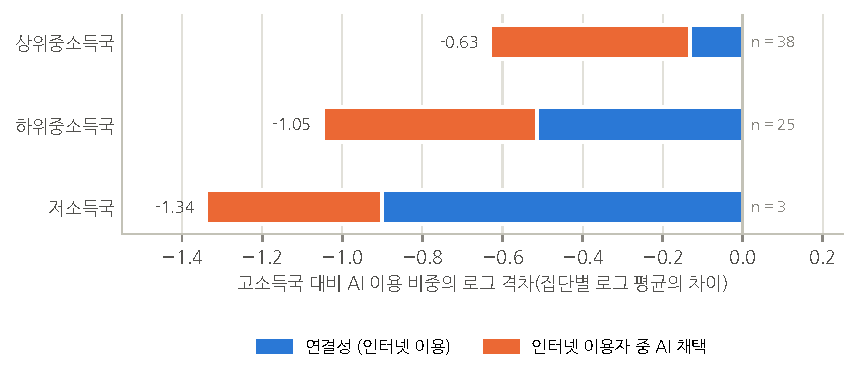
\includegraphics[width=0.9\textwidth]{figures/fig_decomp_ko.pdf}
\caption{고소득국 대비 AI 이용 로그 격차(집단별 로그 비중 평균의 차이)를 연결성(인터넷 이용)과 인터넷 이용자 대비 AI 이용자 비율로 분해한 결과. 마이크로소프트 국가별 추정치, 2026년 2분기. 저소득국 막대는 세 경제권에 기초한다.}\label{fig:decomp}
\end{figure}


\FloatBarrier
\section{추가 표}\label{app:tables}

\begin{table}[ht]
\centering
\begin{threeparttable}
\caption{통제변수를 포함한 AI 이용의 소득 기울기(로그 이용자 비중, 국가별 추정치, 공통 표본)}\label{tab:controls}
\small
\begin{tabular}{@{}lrrrrr@{}}
\toprule
 & (1) & (2) & (3) & (4) & (5) \\
\midrule
\tabinput{tables/tab_controls.tex}
\bottomrule
\end{tabular}
\begin{tablenotes}[flushleft]\footnotesize
\item \emph{주:} OLS, HC3 표준오차. 통제변수는 퍼센트 단위이며, 디지털 결제는 Findex 2025.
\end{tablenotes}
\end{threeparttable}
\end{table}

\begin{table}[ht]
\centering
\begin{threeparttable}
\caption{Anthropic AUI 소득탄력성의 시간적 변화}\label{tab:auitime}
\small
\begin{tabular}{@{}lrrrrrr@{}}
\toprule
 & \multicolumn{4}{c}{기준 충족 전체 경제권} & \multicolumn{2}{c}{공통 표본($N=111$)} \\
\cmidrule(lr){2-5}\cmidrule(lr){6-7}
시점 & 탄력성 & (표준오차) & $N$ & $R^2$ & 탄력성 & (표준오차) \\
\midrule
\tabinput{tables/tab_aui_time.tex}
\bottomrule
\end{tabular}
\begin{tablenotes}[flushleft]\footnotesize
\item \emph{주:} 로그 AUI를 로그 1인당 GNI(2025)에 회귀한 OLS. 표본 대화 200건 이상 경제권(2025년 8월--2026년 2월) 또는 공표값이 있는 경제권(2026년 4--5월). 공통 표본: 다섯 시점 모두 기준을 충족한 경제권. 2025년 8월에서 2026년 2월까지의 변화 0.064(군집 표준오차 0.018), 2026년 2월에서 5월까지의 변화 $-0.006$(0.016).
\end{tablenotes}
\end{threeparttable}
\end{table}

\FloatBarrier % keep the tables of this appendix ahead of the next one
\section{500달러 기준 요금 시나리오}\label{app:500}

2026년 9월 29일의 요금 변경(제~\ref{sec:tariff}절)은 새 고사용량 요금제의 미국 웹 요금을 보여 주지만, 그 요금제의 현지 가격, 세금, 가입 자격 조건은 알려 주지 않는다. 따라서 표~\ref{tab:500}은 20달러와 200달러 기준 요금과 함께 월 500달러라는 공통 요금을 국민소득 표본에 시나리오로 적용한다. 각 나라의 비율을 먼저 계산한 뒤 집단별 중위값을 구한다.

\begin{table}[ht]\centering\begin{threeparttable}
\caption{1인당 GNI 대비 연간 기준 요금}\label{tab:500}
\small\begin{tabular}{lrrrr}\toprule
소득집단 & $N$ & 월 \$20 & 월 \$200 & 월 \$500 \\\midrule
\tabinput{tables/tab_500_scenario.tex}
\bottomrule\end{tabular}
\begin{tablenotes}[flushleft]\footnotesize\item \emph{주:} 각 집단 경제권들의 $1200p/y$(\%) 중위값. 500달러 열은 2026년 9월 29일 발표된 Pro 500 요금제의 웹 요금을 공통 요금으로 적용한 것이며, 이 요금제의 현지 가격은 관측되지 않았다.\end{tablenotes}
\end{threeparttable}\end{table}

월 500달러이면 연간 요금은 6,000달러이며, 2\% 기준에 해당하는 1인당 GNI는 300,000달러로 이에 이르는 경제권은 없다. 부담은 요금에 비례하므로 500달러의 부담은 모든 나라에서 정확히 20달러 부담의 25배다. 이 시나리오는 수준을 키울 뿐, 국가 간 상대적 비율을 바꾸거나 가격 효과를 식별할 수 있는 변동을 더하지 않는다. 또한 무료 요금제나 더 저렴한 요금제가 특정 과업에 충분한지에 대해서도 아무것도 말해 주지 않는다.

\section{접근 조건 기록 프로토콜}\label{app:protocol}

반복 요금만으로 유용한 작업을 마치는 데 드는 비용이 정해지지는 않는다. 접근 조건을 재현 가능하게 관측하려면 국가, 관측 시각, 결제 경로, 사업자, 요금제와 결제 주기, 원래 통화와 세금 표시 방식, 목록 표시와 결제 가능 여부, 가입자 코호트, 기본 사용 허용량과 초기화 규칙, 이용 가능한 모델과 도구, 초과 사용 조건을 기록해야 한다. 알 수 없는 조건은 사업자 전체에 공통인 상수로 채우지 말고 빈칸으로 남겨야 한다. 재현성 패키지는 이러한 관측을 위한 항목 사전(\nolinkurl{publication_upgrade/access_measurement_fields.csv})을 제공한다. 이는 현재 조사를 확장하자는 제안이며, 새로 수집한 자료가 아니다.

미리 정한 작업량 $B$, 품질 규칙 $q$, 기한 $d$에 대해, 국가 $c$와 시점 $t$에서 세 요건을 실제로 모두 충족하는 서비스 구성의 실행 가능 집합을 $\mathcal F(B,q,d;c,t)$라 하자. 최소 현금 지출은 다음과 같다.
\[
C(B,q,d;c,t)=\inf_{a\in\mathcal F(B,q,d;c,t)}\operatorname{cashcost}(a).
\]
이 비교에서는 무료, API, 기관, 로컬 모델 구성을 포함하는지와 고정 하드웨어 비용이나 구독 비용을 어떻게 배분하는지를 밝혀야 한다. 실행 가능성을 판단하려면 정확성, 언어, 모델 버전, 실제 완료 시간, 재시도, 과금된 이용량, 실패를 과업 단위로 관측해야 한다. 이 논문은 이러한 양을 관측하지 않으며 $C$를 추정하지 않는다. 실패한 시도를 빼면 비용이 과소평가되므로, 향후 평가는 성공한 과업당 비용과 함께 총지출과 성공률을 보고해야 한다. 이 프로토콜은 측정된 구독 약정과, 앞으로 품질과 기한 제약 아래에서 관측될 접근 결과를 구분한다.

\end{document}
